%! Author = crist
%! Date = 03/07/2025
\section{Kinematics}
\begin{definition}[Kinematics]
        Is the branch of Physics that studies motion without taking into account the causes that produce it.
\end{definition}
\begin{minipage}{0.45\textwidth}
    \begin{figure}[H]
        \centering
        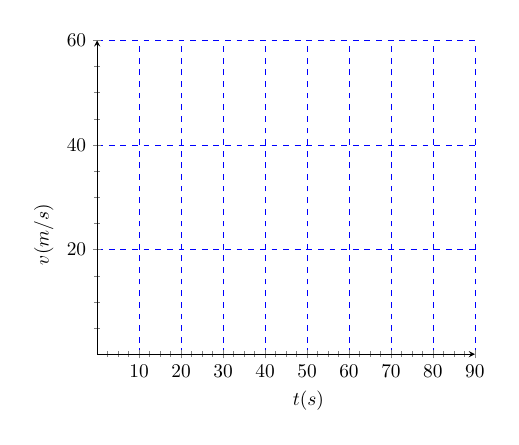
\begin{tikzpicture}[scale=0.7]
                \centering
                \begin{axis}
                    [axis lines = left,
                    axis x line=center,
                    axis y line=center,
                    mark=circle,
% xtick={-5,-4,...,5},
% ytick={-5,-4,...,5},
                    xlabel={$t(s)$},
                    ylabel={$v(m/s)$},
                    ylabel near ticks,
                    xlabel near ticks,
                    xlabel style={below right},
                    ylabel style={above left},
                    ymax=60,
                    ymin=0,
                    xmax=90,
                    xmin=0,
                    xtick={0,10,20,30,40,50,60,70,80,90},
                    ymajorgrids=true,
                    xmajorgrids=true,
                    minor tick num=3,
                    grid style={dashed, blue},
                    ]
                \end{axis}
        \end{tikzpicture}
        \caption{\textbf{Reference system}. Velocity vs. time is represented.}
        \label{fig:reference_system}
    \end{figure}
\end{minipage}
\hfill
\begin{minipage}{0.45\textwidth}
    We say that an object is in motion when its position changes with respect to a reference system over time.

    If its position does not change, we say that the object is at \textbf{rest}.

    Motion is relative, that is, it depends on the point of reference and therefore, for its study, it is necessary to establish a reference system.

    In Physics, the reference system will be a Cartesian coordinate system \( x\ ,\ y \).
\end{minipage}

\vspace*{6pt}
\begin{definition}[Reference System]
         Is a system that allows us to fix the position of an object and study its evolution over time.
\end{definition}

\section{Quantities that describe motion}

To determine motion, we need to know the following quantities:

\begin{enumerate}[label=\numberballmDarkTeal]
        \item \textbf{Position}.
        It tells us the exact location of the object.
        Position is usually represented by the letter \( x \), and its SI unit is the meter (\( \unit{\metre} \)).

        \item \textbf{Displacement}.
        It is the difference between the final position and the initial position of the motion.
        Displacement will be represented as \( \Delta x \):

        \vspace*{20pt}
        \begin{centeredequation}
            \eqnmarkbox[blue]{displacement}{\Delta x}
            =
            \eqnmarkbox[red]{finalpos}{x_f}
            -
            \eqnmarkbox[mygreen]{initialpos}{x_i}
        \end{centeredequation}
        \vspace{25pt}
        \annotate[yshift=1em]{left}{displacement}{Displacement}
        \annotate[yshift=1em]{}{finalpos}{Final position}
        \annotate[yshift=-2em]{below,left}{initialpos}{Initial position}

        Mathematically, the symbol \( \Delta \) indicates the difference between the final and the initial values.

        If this symbol precedes a quantity, it means the final value minus the initial value of that quantity.

        For position, we will have \( \Delta x = x_f - x_i \), for time \( \Delta t = t_f - t_i \), and for velocity \( \Delta v = v_f - v_i \).

         Its unit will also be the meter.

        \begin{remark}
            Here it is important to note that displacement can be \textbf{negative}.
            This occurs when the moving object goes in the opposite direction.
        \end{remark}

        \item \textbf{Trajectory}.
        It is the path followed during the motion.

        \item \textbf{Distance travelled}.
        It is the length of the trajectory.
        Its unit will also be the meter.
\end{enumerate}

Motion can be classified according to its trajectory.
We will therefore have:
\begin{enumerate}[label=\letraminuscula]
        \item \negsubro{Rectilinear}.
        The trajectory is a straight line.
        In this type of motion, displacement coincides with the distance traveled.
        \item \negsubro{Circular}.
        The trajectory is circular.
        \item \negsubro{Curvilinear}.
        The trajectory describes curves.
\end{enumerate}

\begin{exercise}
    In your notebook, identify whether the path (trajectory) of each of the following motions is straight (rectilinear) or curved (circular).
    \begin{enumerate}[label=\letraminuscula]
        \item a ball dropped from a height
        \item a rock attached to a rope and swung in circles
        \item the movement of a clock's second hand
        \item a sprinter racing \qty{100}{\metre} on a straight track
    \end{enumerate}
%    Página 135, Ejericio 11
    \begin{solu}
        \textbf{\textcolor{purple}{Exercise:}} In your notebook, identify whether the path (trajectory) of each of the following motions is straight (rectilinear) or curved (circular).
        \begin{enumerate}[label=\letraminuscula]
            \item a ball dropped from a height
            \item a rock attached to a rope and swung in circles
            \item the movement of a clock's second hand
            \item a sprinter racing \qty{100}{\metre} on a straight track
        \end{enumerate}

        \vspace{0.3cm}

        \begin{enumerate}[label=\letraminuscula]
            \item \textcolor{blue}{Rectilinear (straight line)} - A falling ball moves vertically downward in a straight path due to gravity.
            \item \textcolor{blue}{Circular} - A rock tied to a rope and spun traces a circular trajectory around the center point.
            \item \textcolor{blue}{Circular} - The second hand of a clock moves in a circular path around the clock face.
            \item \textcolor{blue}{Rectilinear (straight line)} - A sprinter running 100 m on a straight track follows a linear path.
        \end{enumerate}
    \end{solu}
\end{exercise}

\begin{exercise}
    Imagine you drive completely around a circular roundabout and arrive back at your starting position. What is your total displacement?
    \begin{solu}
        \textbf{\textcolor{purple}{Exercise:}} Imagine you drive completely around a circular roundabout and arrive back at your starting position. What is your total displacement?

        \vspace{0.3cm}

        \textcolor{red}{Key Concept:} Displacement is a vector quantity that measures the change in position from the initial point to the final point.

        \textcolor{blue}{Given information:}
        \begin{itemize}
            \item Starting position = Final position (you return to where you began)
        \end{itemize}

        \textcolor{blue}{Analysis:}

        Displacement is defined as:
        \[
            \vec{\Delta x} = \vec{x}_{\text{final}} - \vec{x}_{\text{initial}}
        \]

        Since you return to the starting point:
        \[
            \vec{x}_{\text{final}} = \vec{x}_{\text{initial}}
        \]

        Therefore:
        \[
            \vec{\Delta x} = \vec{x}_{\text{initial}} - \vec{x}_{\text{initial}} = \vec{0}
        \]

        \textcolor{red}{Answer:} The displacement is \textbf{zero} (\qty{0}{\m}), even though you traveled a certain distance around the roundabout. This demonstrates the difference between distance (total path length traveled) and displacement (straight-line change in position).
    \end{solu}
\end{exercise}

\begin{exercise}
    If you go all the way around a roundabout and return to the starting point, what’s your displacement?
    \begin{solu}
        Displacement is the straight-line distance between the start and the end.
        \begin{itemize}
            \item \textbf{Initial Position ($x_i$):} Point A.
            \item \textbf{Final Position ($x_f$):} Point A.
            \item \textbf{Calculation:} $\Delta x = x_f - x_i = A - A = \mathbf{0}$.
        \end{itemize}
        The displacement is \textcolor{red}{\qty{0}{\m}}. Note that the \textit{distance travelled} is the perimeter of the roundabout, but the displacement is zero.
    \end{solu}
\end{exercise}


\section{Velocity}

Velocity gives us a measure of how fast an object moves.
We have two types of velocity:

\begin{enumerate}[label=\numberballmDarkTeal]
        \item \textbf{Instantaneous velocity}.
        It is the velocity that an object has at a given moment.
        We can see it in a car's speedometer as the velocity constantly changes.

        \item \textbf{Average velocity}.
        This is the measure of velocity that we will use in this course and we will represent it with the letter \( v \).
        \begin{centeredequation}
            v = \dfrac{\text{Displacement}}{\text{Elapsed time}} = \dfrac{\Delta x}{\Delta t}
        \end{centeredequation}

        \item If we express this in terms of the initial and final position, we have:
        \begin{centeredequation}
            v = \dfrac{x_f - x_i}{t_f - t_i}
        \end{centeredequation}
        \begin{itemize}
            \item \( x_i \) is the initial position.
            \item \( t_i \) is the time measured at the initial position.
            \item \( x_f \) is the final position.
            \item \( t_f \) is the time measured at the final position.
        \end{itemize}
\end{enumerate}

The SI units of velocity are: \unit{\mps}


\section{Acceleration}

Acceleration tells us how velocity changes with time.
Just like velocity, we have two types of acceleration:

\begin{enumerate}[label=\numberballmDarkTeal]
        \item \textbf{Instantaneous acceleration}.
        It is the acceleration at a given instant.

        \item \textbf{Average acceleration}.
        It is the acceleration over a period of time.
        This is the one we will use in this topic.
        The formula is expressed as:
        \begin{centeredequation}
            a = \dfrac{\text{Change in velocity}}{\text{Elapsed time}} = \dfrac{\Delta v}{\Delta t}
        \end{centeredequation}

        \item If we express this in terms of the initial and final velocity, we have:
        \begin{centeredequation}
            a = \dfrac{v_f - v_i}{t_f - t_i}
        \end{centeredequation}
        \begin{itemize}
            \item \( v_i \) is the initial velocity.
            \item \( t_i \) is the time measured at the initial velocity.
            \item \( v_f \) is the final velocity.
            \item \( t_f \) is the time measured at the final velocity.
        \end{itemize}
\end{enumerate}

The SI units of acceleration are: \unit{\mpss}


\section{Rectilinear Motion}

Rectilinear motions are those that have a \textbf{straight-line trajectory}.
These motions are very interesting because in these cases, \textbf{displacement coincides with the distance traveled}.

The previously described equations for velocity and acceleration can be written as:
\begin{centeredequation}
    v = \dfrac{\Delta x}{\Delta t} \longrightarrow v = \dfrac{x_f - x_i}{t_f - t_i}
\end{centeredequation}
\begin{centeredequation}
    a = \dfrac{\Delta v}{\Delta t} \longrightarrow a = \dfrac{v_f - v_i}{t_f - t_i}
\end{centeredequation}
Sometimes these expressions can be simplified because:
\begin{itemize}
    \item Generally, we take \( t_i = 0 \), so this term can be removed.
    We can choose the initial time.
    \item Since there is only one time term left, \( t_f \) can be simplified to just \( t \).
    \item The same applies to \( x_i \), although it is less common.
    If we set the initial position \( x_i = 0 \), it can be removed, and the final position \( x_f \) can simply be called \( x \).
    \item The same simplification can also be applied to \( v_i \).
\end{itemize}
After these simplifications, the equations become:
\begin{centeredequation}
    v = \dfrac{x}{t}
\end{centeredequation}
\begin{centeredequation}
    a = \dfrac{v}{t}
\end{centeredequation}
\begin{remark}
    Even if we can simplify the expressions, it is important to carefully read the problem to see if simplification is allowed.
\end{remark}

\subsection{Uniform Rectilinear Motion (URM)}

This is a specific case of rectilinear motion with the following conditions:
\begin{itemize}
    \item Its trajectory is a straight line.
    \item Its velocity does not change during motion. Therefore:
    \begin{itemize}
        \item \( v_f = v_i \)
        \item \( \Delta v = 0 \)
    \end{itemize}
    \item Since the velocity does not change, acceleration is zero, i.e., \( a = \qty{0}{\mpss} \)

    \begin{theorem}[]
        The velocity is given by: $v = \dfrac{x_f - x_i}{t_f-t_i}$. Applying the previous simplifications: \(  v = \dfrac{x}{t}  \)

%        To find the final position:
%        \begin{centeredequation}
%            x_f = x_i + v\cdot (t_f-t_i)
%        \end{centeredequation}
%        If \( t_i = 0 \):
%        \begin{centeredequation}
%            x_f = x_i + v\cdot t
%        \end{centeredequation}
%        If also \( x_i = 0 \):
%        \begin{centeredequation}
%            x = v\cdot t
%        \end{centeredequation}
%        To find \( t_f \):
%        \begin{centeredequation}
%            t_f = t_i + \dfrac{x_f-x_i}{v}
%        \end{centeredequation}
%        If \( t_i = 0 \):
%        \begin{centeredequation}
%            t = \dfrac{x_f-x_i}{v}
%        \end{centeredequation}
%        If \( x_i = 0 \):
%        \begin{centeredequation}
%            t = \dfrac{x}{v}
%        \end{centeredequation}
    \end{theorem}
\end{itemize}


%    Página 135, Ejericio 12

\begin{exercise}
    The Sun is located at an average distance of \qty{1.5e8}{\kilo\m} from Earth, and the speed of light in a vacuum is \qty{3e8}{\mps}. Assuming light travels at constant velocity (uniform rectilinear motion), calculate how long it takes for light from the Sun to reach Earth.

    \begin{solu}
        \textbf{\textcolor{purple}{Exercise:}} The Sun is located at an average distance of \qty{1.5e8}{\kilo\m} from Earth, and the speed of light in a vacuum is \qty{3e8}{\mps}. Assuming light travels at constant velocity (uniform rectilinear motion), calculate how long it takes for light from the Sun to reach Earth.

        \vspace{0.3cm}

        \textcolor{blue}{Given information:}
        \begin{itemize}
            \item Distance from Sun to Earth: $d = \qty{1.5e8}{\kilo\m}$
            \item Speed of light: $v = \qty{3e8}{\mps}$
            \item Motion type: Uniform rectilinear motion (constant velocity)
        \end{itemize}

        \textcolor{blue}{Step 1: Convert all units to SI (metres and seconds)}
        \[
            d = 1.5 \times 10^8 \text{ km} \times \frac{1000 \text{ m}}{1 \text{ km}} = \textcolor{red}{1.5 \times 10^{11} \text{ m}}
        \]

        \textcolor{blue}{Step 2: Apply the formula for uniform motion}

        For uniform rectilinear motion, the relationship between distance, velocity, and time is:
        \[
            \boxed{d = v \cdot t}
        \]

        \textcolor{blue}{Step 3: Solve for time}

        Rearranging the equation:
        \[
            t = \frac{d}{v}
        \]

        \textcolor{blue}{Step 4: Substitute values and calculate}
        \[
            t = \frac{1.5 \times 10^{11} \text{ m}}{3 \times 10^8 \text{ m/s}} = \frac{1.5}{3} \times 10^{11-8} \text{ s} = 0.5 \times 10^3 \text{ s} = \textcolor{red}{500 \text{ s}}
        \]

        \textcolor{blue}{Step 5: Convert to minutes (optional)}
        \[
            t = 500 \text{ s} \times \frac{1 \text{ min}}{60 \text{ s}} = \textcolor{red}{8.33 \text{ min}} \approx 8 \text{ min } 20 \text{ s}
        \]

        \textcolor{red}{Answer:} It takes light approximately \textbf{500 seconds} (or about \textbf{8 minutes and 20 seconds}) to travel from the Sun to Earth.
    \end{solu}
\end{exercise}


\begin{exercise}
    During a Physical Education lesson, you are timing how long it takes students to run \qty{100}{\m}.
    \begin{enumerate}[label=\letraminuscula]
        \item If one of your classmates completes the \qty{100}{\m} in \qty{15}{\s}, what is her average speed?
        \item On average, how many metres does she cover each second?
    \end{enumerate}
    \begin{solu}
        \textbf{\textcolor{purple}{Exercise:}} During a Physical Education lesson, you are timing how long it takes students to run \qty{100}{\m}.
        \begin{enumerate}[label=\letraminuscula]
            \item If one of your classmates completes the \qty{100}{\m} in \qty{15}{\s}, what is her average speed?
            \item On average, how many metres does she cover each second?
        \end{enumerate}

        \vspace{0.3cm}

        \textcolor{blue}{Given information:}
        \begin{itemize}
            \item Distance: $d = \qty{100}{\m}$
            \item Time: $t = \qty{15}{\s}$
        \end{itemize}

        \textbf{\textcolor{blue}{Part a) Calculate average speed}}

        \textcolor{blue}{Step 1: Apply the average speed formula}

        Average speed is defined as:
        \[
            \boxed{v_{\text{avg}} = \frac{d}{t}}
        \]

        \textcolor{blue}{Step 2: Substitute values and calculate}
        \[
            v_{\text{avg}} = \frac{100 \text{ m}}{15 \text{ s}} = \textcolor{red}{6.67 \text{ m/s}}
        \]

        \textcolor{red}{Answer a):} Her average speed is \textbf{\qty{6.67}{\mps}}.

        \vspace{0.5cm}

        \textbf{\textcolor{blue}{Part b) Metres per second}}

        \textcolor{blue}{Analysis:} The question asks "how many metres does she travel per second," which is exactly the definition of speed in m/s.

        \textcolor{red}{Answer b):} She travels an average of \textbf{6.67 metres per second}. This is the same value as the speed calculated in part a), since speed is measured in metres per second (m/s).
    \end{solu}
\end{exercise}



\begin{exercise}
    During a family road trip, your car travels along a straight motorway at an average speed of \qty{90}{\kmph} for \qty{15}{min}.
    \begin{enumerate}[label=\letraminuscula]
        \item Calculate the distance travelled in metres during this time period.
        \item Can you be certain that the car's speed was exactly \qty{90}{\kmph} at every moment during the journey?
    \end{enumerate}
    \begin{solu}
        \textbf{\textcolor{purple}{Exercise:}} During a family road trip, your car travels along a straight motorway at an average speed of \qty{90}{\kmph} for \qty{15}{min}.
        \begin{enumerate}[label=\letraminuscula]
            \item Calculate the distance travelled in metres during this time period.
            \item Can you be certain that the car's speed was exactly \qty{90}{\kmph} at every moment during the journey?
        \end{enumerate}

        \vspace{0.3cm}

        \textcolor{blue}{Given information:}
        \begin{itemize}
            \item Average speed: $v_{\text{avg}} = \qty{90}{\kmph}$
            \item Time: $t = \qty{15}{min}$
        \end{itemize}

        \textbf{\textcolor{blue}{Part a) Calculate distance in metres}}

        \textcolor{blue}{Step 1: Convert units to SI}

        Convert speed from km/h to m/s:
        \[
            v = 90 \frac{\text{km}}{\text{h}} \times \frac{1000 \text{ m}}{1 \text{ km}} \times \frac{1 \text{ h}}{3600 \text{ s}} = 90 \times \frac{1000}{3600} = \textcolor{red}{25 \text{ m/s}}
        \]

        Convert time from minutes to seconds:
        \[
            t = 15 \text{ min} \times \frac{60 \text{ s}}{1 \text{ min}} = \textcolor{red}{900 \text{ s}}
        \]

        \textcolor{blue}{Step 2: Apply the distance formula}
        \[
            \boxed{d = v \cdot t}
        \]

        \textcolor{blue}{Step 3: Calculate distance}
        \[
            d = 25 \text{ m/s} \times 900 \text{ s} = \textcolor{red}{22,500 \text{ m}}
        \]

        \textcolor{red}{Answer a):} The car travelled \textbf{\qty{22500}{\m}} (or 22.5 km) during those 15 minutes.

        \vspace{0.5cm}

        \textbf{\textcolor{blue}{Part b) Was the speed constant?}}

        \textcolor{blue}{Analysis:} The problem states that 90 km/h is the \textit{average} speed, not the instantaneous speed.

        \textcolor{red}{Answer b):} \textbf{No}, we cannot be certain that the speed was exactly 90 km/h at all times. The value of 90 km/h is the \textit{average speed} over the 15-minute interval. During the journey, the car could have travelled faster or slower at different moments (for example, accelerating to overtake, slowing down for curves, etc.), as long as the average over the entire time period equals 90 km/h.
    \end{solu}
\end{exercise}


\begin{exercise}
    A car moving along a straight highway has been travelling for \qty{30}{min} at an average speed of \qty{100}{\kmph}. What distance, in metres, has the car covered during this time?
    \begin{solu}
        \textbf{\textcolor{purple}{Exercise:}} A car moving along a straight highway has been travelling for \qty{30}{min} at an average speed of \qty{100}{\kmph}. What distance, in metres, has the car covered during this time?

        \vspace{0.3cm}

        \textcolor{blue}{Given information:}
        \begin{itemize}
            \item Average speed: $v_{\text{avg}} = \qty{100}{\kmph}$
            \item Time: $t = \qty{30}{min}$
        \end{itemize}

        \textcolor{blue}{Step 1: Convert units to SI}

        Convert speed from km/h to m/s:
        \[
            v = 100 \frac{\text{km}}{\text{h}} \times \frac{1000 \text{ m}}{1 \text{ km}} \times \frac{1 \text{ h}}{3600 \text{ s}} = 100 \times \frac{1000}{3600} = \textcolor{red}{27.78 \text{ m/s}}
        \]

        Convert time from minutes to seconds:
        \[
            t = 30 \text{ min} \times \frac{60 \text{ s}}{1 \text{ min}} = \textcolor{red}{1800 \text{ s}}
        \]

        \textcolor{blue}{Step 2: Apply the distance formula for uniform motion}
        \[
            \boxed{d = v \cdot t}
        \]

        \textcolor{blue}{Step 3: Substitute values and calculate}
        \[
            d = 27.78 \text{ m/s} \times 1800 \text{ s} = \textcolor{red}{50,000 \text{ m}}
        \]

        \textcolor{red}{Answer:} The car has travelled \textbf{\qty{50000}{\m}} (or 50 km) during the 30 minutes.
    \end{solu}
\end{exercise}


\begin{exercise}
    A car is moving along a straight road, and its velocity changes as follows: After \qty{1}{\s}, its velocity is \qty{2}{\mps}. After \qty{2}{\s} from the start, its velocity is \qty{4}{\mps}. After \qty{3}{\s}, its velocity is \qty{6}{\mps}.

    \begin{enumerate}[label=\letraminuscula]
        \item By how much does the car's velocity change during each second?
        \item What is the acceleration of this vehicle?
    \end{enumerate}
    \begin{solu}
        \textbf{\textcolor{purple}{Exercise:}} A car is moving along a straight road, and its velocity changes as follows: After \qty{1}{\s}, its velocity is \qty{2}{\mps}. After \qty{2}{\s} from the start, its velocity is \qty{4}{\mps}. After \qty{3}{\s}, its velocity is \qty{6}{\mps}.
        \begin{enumerate}[label=\letraminuscula]
            \item By how much does the car's velocity change during each second?
            \item What is the acceleration of this vehicle?
        \end{enumerate}

        \vspace{0.3cm}

        \textcolor{blue}{Given information:}
        \begin{itemize}
            \item At $t_1 = 1$ s: $v_1 = \qty{2}{\mps}$
            \item At $t_2 = 2$ s: $v_2 = \qty{4}{\mps}$
            \item At $t_3 = 3$ s: $v_3 = \qty{6}{\mps}$
        \end{itemize}

        \textbf{\textcolor{blue}{Part a) Velocity change per second}}

        \textcolor{blue}{Step 1: Calculate velocity changes}

        Change during the first second (from $t=0$ to $t=1$ s):
        \[
            \Delta v_1 = v_1 - v_0 = 2 - 0 = \textcolor{red}{2 \text{ m/s}}
        \]

        Change during the second second (from $t=1$ to $t=2$ s):
        \[
            \Delta v_2 = v_2 - v_1 = 4 - 2 = \textcolor{red}{2 \text{ m/s}}
        \]

        Change during the third second (from $t=2$ to $t=3$ s):
        \[
            \Delta v_3 = v_3 - v_2 = 6 - 4 = \textcolor{red}{2 \text{ m/s}}
        \]

        \textcolor{red}{Answer a):} The car's velocity increases by \textbf{\qty{2}{\mps}} during each second.

        \vspace{0.5cm}

        \textbf{\textcolor{blue}{Part b) Calculate acceleration}}

        \textcolor{blue}{Step 2: Apply the acceleration formula}

        Acceleration is defined as the rate of change of velocity:
        \[
            \boxed{a = \frac{\Delta v}{\Delta t}}
        \]

        Since the velocity changes by 2 m/s every 1 second:
        \[
            a = \frac{2 \text{ m/s}}{1 \text{ s}} = \textcolor{red}{2 \text{ m/s}^2}
        \]

        \textcolor{blue}{Alternative calculation using any two points:}
        \[
            a = \frac{v_3 - v_1}{t_3 - t_1} = \frac{6 - 2}{3 - 1} = \frac{4}{2} = \textcolor{red}{2 \text{ m/s}^2}
        \]

        \textcolor{red}{Answer b):} The acceleration of the vehicle is \textbf{\qty{2}{\metre\per\second\squared}}.

        \textcolor{blue}{Note:} Since the acceleration is constant and positive, this is uniformly accelerated motion.
    \end{solu}
\end{exercise}

\begin{exercise}
    A cyclist leaves Almansa on the bike lane at a speed of \qty{8}{\mps}.
    If it takes \qty{100}{\min} to reach his destination:
    \begin{enumerate}[label=\letraminuscula]
    \item What distance has he travelled?
    \item Knowing that Bonete is \qty{32}{\km} away, how long would it take him?
    \end{enumerate}
\end{exercise}

\subsubsection{Graphs of Uniform Rectilinear Motion (URM)}
In physics, it is very common to make graphs and from them identify the type of motion. For URM, we will have the following cases.
\begin{figure}[H]
    \centering
    % First subfigure
    \begin{subfigure}[b]{0.45\textwidth}
        \centering
        \begin{tikzpicture}[scale=0.85]
            \begin{axis}
                [
                ylabel={$x$ (\unit{\m})},
                xlabel={$t$ (\unit{\s})},
                axis lines=middle,
                enlargelimits=true,
                xmin=0, xmax=10,
                ymin=0, ymax=10,
                domain=0:8,
                samples=100,
                legend pos=outer north east,
                legend style={draw=none},
                xticklabels={},
                yticklabels={}
                ]
                \addplot[line width=1.5pt, red] {3 + 0.5*x};
            \end{axis}
        \end{tikzpicture}
        \caption{Position vs Time. Moving in the positive direction.}
    \end{subfigure}
    \hfill
    % Second subfigure
    \begin{subfigure}[b]{0.45\textwidth}
        \centering
        \begin{tikzpicture}[scale=0.85]
            \begin{axis}
                [
                ylabel={$x$ (\unit{\m})},
                xlabel={$t$ (\unit{\s})},
                axis lines=middle,
                enlargelimits=true,
                xmin=0, xmax=10,
                ymin=0, ymax=10,
                domain=0:8,
                samples=100,
                legend pos=outer north east,
                legend style={draw=none},
                xticklabels={},
                yticklabels={}
                ]
                \addplot[line width=1.5pt, red] {8 - 0.5*x};
            \end{axis}
        \end{tikzpicture}
        \caption{Position vs Time. Moving in the opposite direction.}
    \end{subfigure}
\end{figure}

\begin{figure}[H]
    \centering
    % First subfigure
    \begin{subfigure}[b]{0.45\textwidth}
        \centering
        \begin{tikzpicture}[scale=0.85]
            \begin{axis}
                [
                ylabel={$v$ (\unit{\mps})},
                xlabel={$t$ (\unit{\s})},
                axis lines=middle,
                enlargelimits=true,
                xmin=0, xmax=10,
                ymin=0, ymax=10,
                domain=0:8,
                samples=100,
                legend pos=outer north east,
                legend style={draw=none},
                xticklabels={},
                yticklabels={}
                ]
                \addplot[line width=1.5pt, red] {5};
            \end{axis}
        \end{tikzpicture}
        \caption{Velocity vs Time. Moving in the positive direction.}
    \end{subfigure}
    \hfill
    % Second subfigure
    \begin{subfigure}[b]{0.45\textwidth}
        \centering
        \begin{tikzpicture}[scale=0.85]
            \begin{axis}
                [
                ylabel={$a$ (\unit{\mpss})},
                xlabel={$t$ (\unit{\s})},
                axis lines=middle,
                enlargelimits=true,
                xmin=0, xmax=10,
                ymin=-1, ymax=10,
                domain=0:8,
                samples=100,
                legend style={draw=none},
                xticklabels={},
                yticklabels={}
                ]
                \addplot[line width=2pt, red] {0};
            \end{axis}
        \end{tikzpicture}
        \caption{Acceleration vs Time.}
    \end{subfigure}
\end{figure}
%\begin{remark}
%    If the motion is in the opposite direction, the velocity vs time graph would look like:
%    \begin{figure}[H]
%        \centering
%        \begin{tikzpicture}[scale=0.85]
%            \begin{axis}
%                [
%                ylabel={$v$ (\unit{\mps})},
%                xlabel={$t$ (\unit{\s})},
%                axis lines=middle,
%                enlargelimits=true,
%                xmin=-10, xmax=2,
%                ymin=0, ymax=10,
%                domain=-10:2,
%                samples=100,
%                legend pos=outer north east,
%                legend style={draw=none},
%                xticklabels={},
%                yticklabels={}
%                ]
%                \addplot[line width=1.5pt, red] {-5};
%            \end{axis}
%        \end{tikzpicture}
%        \caption{Velocity vs Time. Moving in the opposite direction.}
%    \end{figure}
%\end{remark}


\subsection{Uniformly Accelerated Rectilinear Motion (UARM)}

This is another specific case of rectilinear motion that meets the following conditions:
\begin{itemize}
    \item The trajectory is also in a straight line.
    \item Now, the velocity changes during the motion.
    \begin{itemize}
        \item \( v_f \neq v_i \)
        \item \( \Delta v \neq  0 \)
    \end{itemize}
    \item Since the velocity changes, the acceleration is now different from zero (\( a \neq 0 \)) but constant, meaning the acceleration does not vary.
\end{itemize}

The equations for this motion are as follows:
\begin{itemize}
    \item For acceleration we have:
    \begin{centeredequation}
        a = \dfrac{v_f - v_i}{t_f - t_i} \label{eq:aceleracion_general}
    \end{centeredequation}
    If we apply the simplifications \( v_i = 0 \) and \( t_i = 0 \), we get:
    \begin{centeredequation}
        a = \dfrac{v}{t}
    \end{centeredequation}
    \item The equation for position is:
    \begin{centeredequation}
        x_f = x_i + v_i\cdot (t_f - t_i) + \frac{1}{2} \cdot a \cdot (t_f - t_i)^2 \label{eq:posición_general}
    \end{centeredequation}
    If we simplify by assuming initial time \( t_i = 0 \), the equation becomes:
    \begin{centeredequation}
        x_f = x_i + v_i \cdot t + \frac{1}{2} \cdot a \cdot t^2
    \end{centeredequation}
    If we also assume the initial position is zero (\( x_i = 0 \)), this expression simplifies further:
    \begin{centeredequation}
        x = v_i \cdot t + \frac{1}{2} \cdot a \cdot t^2
    \end{centeredequation}
    As we can see, in this equation \( v_f \) never appears, which means that the final position does not depend on the final velocity, but it does depend on the initial velocity since it appears in the formula.
    \item Due to the complexity of solving for time in this type of motion, the expression will not be studied in this course.
\end{itemize}


\begin{exercise}
    You have gone skiing with your classmates and decide to go down a slope. Starting from rest, you accelerate to \qty{10}{\mps} in \qty{5}{\s}. What was your average acceleration?
    \begin{solu}
        \textbf{\textcolor{purple}{Exercise:}} You have gone skiing with your classmates and decide to go down a slope. Starting from rest, you accelerate to \qty{10}{\mps} in \qty{5}{\s}. What was your average acceleration?

        \vspace{0.3cm}

        \textcolor{blue}{Given information:}
        \begin{itemize}
            \item Initial velocity: $v_0 = \qty{0}{\mps}$ (starting from rest)
            \item Final velocity: $v_f = \qty{10}{\mps}$
            \item Time interval: $\Delta t = \qty{5}{\s}$
        \end{itemize}

        \textcolor{blue}{Step 1: Apply the acceleration formula}

        Acceleration is defined as the change in velocity divided by the time interval:
        \[
            \boxed{a = \frac{\Delta v}{\Delta t} = \frac{v_f - v_0}{\Delta t}}
        \]

        \textcolor{blue}{Step 2: Calculate the change in velocity}
        \[
            \Delta v = v_f - v_0 = 10 - 0 = \textcolor{red}{10 \text{ m/s}}
        \]

        \textcolor{blue}{Step 3: Calculate acceleration}
        \[
            a = \frac{10 \text{ m/s}}{5 \text{ s}} = \textcolor{red}{2 \text{ m/s}^2}
        \]

        \textcolor{red}{Answer:} Your average acceleration down the slope was \textbf{\qty{2}{\metre\per\second\squared}}.

        \textcolor{blue}{Physical interpretation:} This means that your velocity increased by 2 m/s every second during the descent.
    \end{solu}
\end{exercise}


\begin{exercise}
    A vehicle accelerates from rest to \qty{100}{\kmph} in \qty{8}{\s}. Calculate its average acceleration, giving your answer in \unit{\mpss}.
    \begin{solu}
        \textbf{\textcolor{purple}{Exercise:}} A vehicle accelerates from rest to \qty{100}{\kmph} in \qty{8}{\s}. Calculate its average acceleration, giving your answer in \unit{\mpss}.

        \vspace{0.3cm}

        \textcolor{blue}{Given information:}
        \begin{itemize}
            \item Initial velocity: $v_0 = \qty{0}{\kmph}$ (from rest)
            \item Final velocity: $v_f = \qty{100}{\kmph}$
            \item Time interval: $\Delta t = \qty{8}{\s}$
        \end{itemize}

        \textcolor{blue}{Step 1: Convert velocity to m/s}

        Initial velocity (already zero in any units):
        \[
            v_0 = 0 \text{ m/s}
        \]

        Final velocity:
        \[
            v_f = 100 \frac{\text{km}}{\text{h}} \times \frac{1000 \text{ m}}{1 \text{ km}} \times \frac{1 \text{ h}}{3600 \text{ s}} = 100 \times \frac{1000}{3600} = \textcolor{red}{27.78 \text{ m/s}}
        \]

        \textcolor{blue}{Step 2: Apply the acceleration formula}
        \[
            \boxed{a = \frac{\Delta v}{\Delta t} = \frac{v_f - v_0}{\Delta t}}
        \]

        \textcolor{blue}{Step 3: Calculate the change in velocity}
        \[
            \Delta v = v_f - v_0 = 27.78 - 0 = \textcolor{red}{27.78 \text{ m/s}}
        \]

        \textcolor{blue}{Step 4: Calculate acceleration}
        \[
            a = \frac{27.78 \text{ m/s}}{8 \text{ s}} = \textcolor{red}{3.47 \text{ m/s}^2}
        \]

        \textcolor{red}{Answer:} The average acceleration of the vehicle is \textbf{\qty{3.47}{\metre\per\second\squared}}.

        \textcolor{blue}{Physical interpretation:} The vehicle's velocity increases by approximately 3.47 m/s every second during the acceleration period.
    \end{solu}
\end{exercise}


\begin{exercise}
    A car travelling at \qty{30}{\mps} applies the brakes for \qty{5}{\s}, reducing its velocity to \qty{25}{\mps}. Determine its average acceleration during braking.
    \begin{solu}
        \textbf{\textcolor{purple}{Exercise:}} A car travelling at \qty{30}{\mps} applies the brakes for \qty{5}{\s}, reducing its velocity to \qty{25}{\mps}. Determine its average acceleration during braking.

        \vspace{0.3cm}

        \textcolor{blue}{Given information:}
        \begin{itemize}
            \item Initial velocity: $v_0 = \qty{30}{\mps}$
            \item Final velocity: $v_f = \qty{25}{\mps}$
            \item Time interval: $\Delta t = \qty{5}{\s}$
        \end{itemize}

        \textcolor{blue}{Step 1: Apply the acceleration formula}
        \[
            \boxed{a = \frac{\Delta v}{\Delta t} = \frac{v_f - v_0}{\Delta t}}
        \]

        \textcolor{blue}{Step 2: Calculate the change in velocity}
        \[
            \Delta v = v_f - v_0 = 25 - 30 = \textcolor{red}{-5 \text{ m/s}}
        \]

        \textcolor{blue}{Note:} The change in velocity is negative because the car is slowing down.

        \textcolor{blue}{Step 3: Calculate acceleration}
        \[
            a = \frac{-5 \text{ m/s}}{5 \text{ s}} = \textcolor{red}{-1 \text{ m/s}^2}
        \]

        \textcolor{red}{Answer:} The average acceleration during braking is \textbf{\qty{-1}{\metre\per\second\squared}}.

        \textcolor{blue}{Physical interpretation:} The negative sign indicates that this is a deceleration (the car is slowing down). The magnitude of the acceleration is 1 m/s², meaning the car's velocity decreases by 1 m/s every second during braking.
    \end{solu}
\end{exercise}


\begin{exercise}
    For take-off, an Airbus aircraft needs to reach a speed of \qty{300}{\kmph} in a time of \qty{23.8}{\s}. Calculate:
    \begin{enumerate}[label=\letraminuscula]
    \item What is its acceleration?
    \item What is the minimum length of runway required?
    \end{enumerate}
    \begin{solu}
        \textbf{\textcolor{purple}{Exercise:}} For take-off, an Airbus aircraft needs to reach a speed of \qty{300}{\kmph} in a time of \qty{23.8}{\s}. Calculate:
        \begin{enumerate}[label=\letraminuscula]
            \item What is its acceleration?
            \item What is the minimum length of runway required?
        \end{enumerate}

        \vspace{0.3cm}

        \textcolor{blue}{Given information:}
        \begin{itemize}
            \item Initial velocity: $v_0 = \qty{0}{\kmph}$ (starts from rest)
            \item Final velocity: $v_f = \qty{300}{\kmph}$
            \item Time: $t = \qty{23.8}{\s}$
        \end{itemize}

        \textbf{\textcolor{blue}{Part a) Calculate acceleration}}

        \textcolor{blue}{Step 1: Convert velocity to m/s}
        \[
            v_0 = 0 \text{ m/s}
        \]
        \[
            v_f = 300 \frac{\text{km}}{\text{h}} \times \frac{1000 \text{ m}}{1 \text{ km}} \times \frac{1 \text{ h}}{3600 \text{ s}} = 300 \times \frac{1000}{3600} = \textcolor{red}{83.33 \text{ m/s}}
        \]

        \textcolor{blue}{Step 2: Apply the acceleration formula}
        \[
            \boxed{a = \frac{v_f - v_0}{t}}
        \]

        \textcolor{blue}{Step 3: Calculate acceleration}
        \[
            a = \frac{83.33 - 0}{23.8} = \frac{83.33}{23.8} = \textcolor{red}{3.50 \text{ m/s}^2}
        \]

        \textcolor{red}{Answer a):} The acceleration is \textbf{\qty{3.50}{\metre\per\second\squared}}.

        \vspace{0.5cm}

        \textbf{\textcolor{blue}{Part b) Calculate runway length}}

        \textcolor{blue}{Step 4: Apply the kinematic equation for distance}

        For uniformly accelerated motion starting from rest, we can use:
        \[
            \boxed{d = v_0 \cdot t + \frac{1}{2} a t^2}
        \]

        Or alternatively:
        \[
            \boxed{v_f^2 = v_0^2 + 2ad} \Rightarrow d = \frac{v_f^2 - v_0^2}{2a}
        \]

        \textcolor{blue}{Method 1: Using $d = v_0 t + \frac{1}{2}at^2$}
        \[
            d = 0 \times 23.8 + \frac{1}{2} \times 3.50 \times (23.8)^2
        \]
        \[
            d = 0 + \frac{1}{2} \times 3.50 \times 566.44 = 1.75 \times 566.44 = \textcolor{red}{991.27 \text{ m}}
        \]

        \textcolor{blue}{Method 2: Using $d = \frac{v_f^2 - v_0^2}{2a}$}
        \[
            d = \frac{(83.33)^2 - 0^2}{2 \times 3.50} = \frac{6943.89}{7.00} = \textcolor{red}{991.98 \text{ m}}
        \]

        \textcolor{red}{Answer b):} The minimum runway length required is approximately \textbf{\qty{992}{\m}} (or about 1 km).

        \textcolor{blue}{Note:} Both methods give essentially the same result; small differences are due to rounding during calculations.
    \end{solu}
\end{exercise}


\begin{exercise}
    A motorcyclist travelling at \qty{20}{\mps} sees a traffic light turn red ahead. He begins braking and comes to a complete stop in \qty{10}{\s}.
    \begin{enumerate}[label=\letraminuscula]
    \item Calculate the acceleration during braking.
    \item If the traffic light was \qty{90}{\m} away from the motorcyclist when he started braking, does he manage to stop before reaching it?
    \end{enumerate}
    \begin{solu}
        \textbf{\textcolor{purple}{Exercise:}} A motorcyclist travelling at \qty{20}{\mps} sees a traffic light turn red ahead. He begins braking and comes to a complete stop in \qty{10}{\s}.
        \begin{enumerate}[label=\letraminuscula]
            \item Calculate the acceleration during braking.
            \item If the traffic light was \qty{90}{\m} away from the motorcyclist when he started braking, does he manage to stop before reaching it?
        \end{enumerate}

        \vspace{0.3cm}

        \textcolor{blue}{Given information:}
        \begin{itemize}
            \item Initial velocity: $v_0 = \qty{20}{\mps}$
            \item Final velocity: $v_f = \qty{0}{\mps}$ (comes to a stop)
            \item Time: $t = \qty{10}{\s}$
            \item Distance to traffic light: $d_{\text{light}} = \qty{90}{\m}$
        \end{itemize}

        \textbf{\textcolor{blue}{Part a) Calculate braking acceleration}}

        \textcolor{blue}{Step 1: Apply the acceleration formula}
        \[
            \boxed{a = \frac{v_f - v_0}{t}}
        \]

        \textcolor{blue}{Step 2: Calculate acceleration}
        \[
            a = \frac{0 - 20}{10} = \frac{-20}{10} = \textcolor{red}{-2 \text{ m/s}^2}
        \]

        \textcolor{red}{Answer a):} The braking acceleration is \textbf{\qty{-2}{\metre\per\second\squared}}.

        \textcolor{blue}{Note:} The negative sign indicates deceleration (slowing down).

        \vspace{0.5cm}

        \textbf{\textcolor{blue}{Part b) Does he stop before the traffic light?}}

        \textcolor{blue}{Step 3: Calculate braking distance}

        Using the kinematic equation:
        \[
            \boxed{d = v_0 \cdot t + \frac{1}{2} a t^2}
        \]

        \textcolor{blue}{Step 4: Substitute values}
        \[
            d_{\text{braking}} = 20 \times 10 + \frac{1}{2} \times (-2) \times (10)^2
        \]
        \[
            d_{\text{braking}} = 200 + \frac{1}{2} \times (-2) \times 100
        \]
        \[
            d_{\text{braking}} = 200 - 100 = \textcolor{red}{100 \text{ m}}
        \]

        \textcolor{blue}{Alternative method using: $v_f^2 = v_0^2 + 2ad$}
        \[
            0^2 = 20^2 + 2 \times (-2) \times d
        \]
        \[
            0 = 400 - 4d
        \]
        \[
            d = \frac{400}{4} = \textcolor{red}{100 \text{ m}}
        \]

        \textcolor{blue}{Step 5: Compare distances}
        \[
            d_{\text{braking}} = 100 \text{ m} > d_{\text{light}} = 90 \text{ m}
        \]

        \textcolor{red}{Answer b):} \textbf{No}, the motorcyclist does \textbf{not} manage to stop in time. He needs 100 m to come to a complete stop, but the traffic light is only 90 m away. He would pass the red light by 10 m before stopping.

        \textcolor{blue}{Safety note:} This demonstrates the importance of maintaining safe following distances and being aware of stopping distances at different speeds.
    \end{solu}
\end{exercise}



\begin{exercise}
    In an experiment, we measure the position of a cart moving along a straight line at different times. The recorded data shows the times when the cart passes through various positions.
    \begin{table}[H]
        \centering
        \renewcommand{\arraystretch}{1.5}
        \begin{tabular}{Occcc}
            \bottomrule
            \textcolor{ocre}{\textbf{Position (\unit{\metre})}} & 0 & 3 & 6 & 9 \\
            \hline
            \textcolor{ocre}{\textbf{Time (\unit{\s})}}         & 0 & 1 & 2 & 3 \\
            \toprule
        \end{tabular}
        \label{tab:ejercicio1}
    \end{table}
%    \begin{figure}[H]
%        \centering
%        \includegraphics[scale=0.8]{images/cinematica/ejercicio_40}
%    \end{figure}
    \begin{enumerate}[label=\letraminuscula]
    \item Draw the position-time graph.
    \item What position does the cart occupy relative to the origin after \qty{3.5}{\s}?
    \item At what instant is the cart \qty{7}{\m} from its initial position?
    \end{enumerate}

    \begin{solu}
        \textbf{\textcolor{purple}{Exercise:}} In an experiment, we measure the position of a cart moving along a straight line at different times. The recorded data shows the times when the cart passes through various positions.
        \begin{enumerate}[label=\letraminuscula]
            \item Draw the position-time graph.
            \item What position does the cart occupy relative to the origin after \qty{3.5}{\s}?
            \item At what instant is the cart \qty{7}{\m} from its initial position?
        \end{enumerate}

        \vspace{0.3cm}

        \textcolor{red}{Note:} Since the actual data from the figure is not visible in the text, I'll provide a general solution method. You would need to read the specific values from the table/figure in your book.

        \textbf{\textcolor{blue}{Part a) Drawing the position-time graph}}

        \textcolor{blue}{Steps:}
        \begin{enumerate}
            \item Create a coordinate system with time ($t$) on the horizontal axis and position ($x$) on the vertical axis.
            \item Mark the data points from the table (time, position) on the graph.
            \item Connect the points. If they form a straight line, the motion is uniform. If they form a curve, the motion is accelerated.
        \end{enumerate}

        \textbf{\textcolor{blue}{Part b) Position at $t = 3.5$ s}}

        \textcolor{blue}{Method:}
        \begin{itemize}
            \item Locate $t = 3.5$ s on the time axis
            \item Draw a vertical line up to the graph
            \item Read the corresponding position value on the vertical axis
            \item If the point falls between data points, interpolate or use the equation of motion
        \end{itemize}

        \textcolor{blue}{If the motion is uniform:} Use $x = x_0 + vt$ where $v$ is the constant velocity calculated from any two points.

        \textcolor{blue}{If the motion is uniformly accelerated:} Use $x = x_0 + v_0 t + \frac{1}{2}at^2$

        \textbf{\textcolor{blue}{Part c) Time when cart is 7 m from initial position}}

        \textcolor{blue}{Method:}
        \begin{itemize}
            \item Find $x = x_0 + 7$ m on the position axis
            \item Draw a horizontal line to intersect the graph
            \item Read the corresponding time value on the horizontal axis
            \item Alternatively, solve the equation of motion for $t$ when $x = x_0 + 7$
        \end{itemize}

        \textcolor{red}{To complete this exercise fully, please refer to the specific data in the figure and apply these methods.}
    \end{solu}
\end{exercise}

\begin{exercise}
    A car at \qty{30}{\mps} brakes for 5 s until it reaches \qty{25}{\mps}. Acceleration?
    \begin{solu}
        $v_i = 30$; $v_f = 25$; $t = 5$. \\
        $a = \frac{25 - 30}{5} = \frac{-5}{5} = \mathbf{-1\,m/s^2}$. (Deceleration).
    \end{solu}
\end{exercise}


\begin{exercise}
    An athlete runs along a straight, horizontal track. Her progress is measured and recorded in the table shown below:
    \begin{table}[H]
        \centering
        \renewcommand{\arraystretch}{1.5}
        \begin{tabular}{Occccc}
            \bottomrule
            \textcolor{ocre}{\textbf{Distance (\unit{\metre})}} & 0 & 30 & 60 & 90 & 120 \\
            \hline
            \textcolor{ocre}{\textbf{Time (\unit{\s})}}         & 0 & 5  & 10 & 15 & 20  \\
            \toprule
        \end{tabular}
        \label{tab:ejercicio2}
    \end{table}
%    \begin{figure}[H]
%        \centering
%        \includegraphics[scale=0.8]{images/cinematica/ejercicio_15}
%    \end{figure}

    \begin{enumerate}[label=\letraminuscula]
    \item Draw the position-time graph.
    \item Calculate the athlete's average speed. What distance has she covered during the first eight seconds?
    \item How long does it take her to travel \qty{66}{\m}?
    \item Does the athlete's instantaneous velocity differ from the average speed at any of the measured time points? What type of motion does your answer suggest?
    \end{enumerate}

    \begin{solu}
        \textbf{\textcolor{purple}{Exercise:}} An athlete runs along a straight, horizontal track. Her progress is measured and recorded in the table shown below:
        \begin{enumerate}[label=\letraminuscula]
            \item Draw the position-time graph.
            \item Calculate the athlete's average speed. What distance has she covered during the first eight seconds?
            \item How long does it take her to travel \qty{66}{\m}?
            \item Does the athlete's instantaneous velocity differ from the average speed at any of the measured time points? What type of motion does your answer suggest?
        \end{enumerate}

        \vspace{0.3cm}

        \textcolor{red}{Note:} Since the specific data table is not provided in the text, I'll demonstrate the solution method. Please use the actual values from your textbook's table.

        \textcolor{blue}{Assuming typical data for this type of exercise might be:}
        \begin{center}
            % --- tabla antigua ---
            % \begin{tabular}{|c|c|c|c|c|c|}
                % \hline
                % \textbf{Time (s)}     & 0 & 2    & 4  & 6    & 8  \\
                % \hline
                % \textbf{Position (m)} & 0 & 16.5 & 33 & 49.5 & 66 \\
                % \hline
            % \end{tabular}
            % --- tabla nueva ---
            \begin{tabular}{@{}cccccc@{}}
                \toprule
                \textbf{Time (s)} & \textbf{0} & \textbf{2} & \textbf{4} & \textbf{6} & \textbf{8} \\
                \midrule
                \textbf{Position (m)} & 0 & 16.5 & 33 & 49.5 & 66 \\
                \bottomrule
            \end{tabular}
        \end{center}

        \textbf{\textcolor{blue}{Part a) Position-time graph}}

        \textcolor{blue}{Steps:}
        \begin{itemize}
            \item Plot time on the x-axis and position on the y-axis
            \item Mark each data point
            \item Connect the points
            \item If the points form a straight line through the origin, the motion is uniform
        \end{itemize}

        \textbf{\textcolor{blue}{Part b) Average speed and distance in 8 seconds}}

        \textcolor{blue}{Step 1: Calculate average speed}
        \[
            \boxed{v_{\text{avg}} = \frac{\Delta x}{\Delta t} = \frac{x_f - x_0}{t_f - t_0}}
        \]

        Using the assumed data:
        \[
            v_{\text{avg}} = \frac{66 - 0}{8 - 0} = \frac{66}{8} = \textcolor{red}{8.25 \text{ m/s}}
        \]

        \textcolor{blue}{Step 2: Distance travelled in first 8 seconds}

        Distance = final position - initial position = $66 - 0 = \textcolor{red}{66 \text{ m}}$

        \textcolor{red}{Answer b):} Average speed is \textbf{8.25 m/s}, and she travelled \textbf{66 m} in 8 seconds.

        \textbf{\textcolor{blue}{Part c) Time to travel 66 m}}

        From the table (or graph), when position = 66 m, time = \textcolor{red}{8 s}

        \textcolor{red}{Answer c):} It takes \textbf{8 seconds} to travel 66 m.

        \textbf{\textcolor{blue}{Part d) Type of motion}}

        \textcolor{blue}{Analysis:} Calculate instantaneous velocities between consecutive points:

        Between 0 and 2 s:
        \[
            v_1 = \frac{16.5 - 0}{2 - 0} = \frac{16.5}{2} = 8.25 \text{ m/s}
        \]

        Between 2 and 4 s:
        \[
            v_2 = \frac{33 - 16.5}{4 - 2} = \frac{16.5}{2} = 8.25 \text{ m/s}
        \]

        Between 4 and 6 s:
        \[
            v_3 = \frac{49.5 - 33}{6 - 4} = \frac{16.5}{2} = 8.25 \text{ m/s}
        \]

        Between 6 and 8 s:
        \[
            v_4 = \frac{66 - 49.5}{8 - 6} = \frac{16.5}{2} = 8.25 \text{ m/s}
        \]

        \textcolor{red}{Answer d):} \textbf{No}, the instantaneous velocity does \textbf{not} differ from the average speed at any measured point. All velocity values are equal to 8.25 m/s. This indicates \textbf{uniform rectilinear motion} (constant velocity), where the athlete runs at a steady pace throughout the measurement period.

        \textcolor{blue}{Remember to use the actual data from your textbook table!}
    \end{solu}
\end{exercise}


\begin{exercise}
%Exercise 52
    In an experiment, we measure different positions of a cart over time and get the results shown in the table below.

    \begin{table}[H]
        \centering
        \renewcommand{\arraystretch}{1.5}
        \begin{tabular}{Occcc}
            \bottomrule
            \textcolor{ocre}{\textbf{Position (\unit{\metre})}} & 0 & 5 & 15 & 25 \\
            \hline
            \textcolor{ocre}{\textbf{Time (\unit{\s})}}         & 0 & 5 & 10 & 15 \\
            \toprule
        \end{tabular}
        \label{tab:ejercicio1}
    \end{table}
%
%    \begin{figure}[H]
%        \centering
%        \includegraphics[scale=0.8]{images/cinematica/ejercicio_52}
%    \end{figure}
    \begin{solu}
        \textbf{\textcolor{purple}{Exercise:}} In an experiment, we measure different positions of a cart over time and obtain the results shown in the figure below.

        \vspace{0.3cm}

        \textcolor{red}{Note:} Without seeing the specific data in the figure, here's the general approach:

        \textcolor{blue}{Steps for analysis:}

        \textbf{1. Identify the type of motion:}
        \begin{itemize}
            \item If the position-time graph is a straight line: \textcolor{red}{uniform motion} (constant velocity)
            \item If the graph is a parabola (curved): \textcolor{red}{uniformly accelerated motion}
        \end{itemize}

        \textbf{2. For uniform motion:}
        \begin{itemize}
            \item Calculate velocity: $v = \frac{\Delta x}{\Delta t}$ (slope of the line)
            \item Write equation: $x = x_0 + vt$
        \end{itemize}

        \textbf{3. For uniformly accelerated motion:}
        \begin{itemize}
            \item Calculate acceleration from: $a = \frac{\Delta v}{\Delta t}$ or analyze the curvature
            \item Determine initial velocity $v_0$ and initial position $x_0$
            \item Write equation: $x = x_0 + v_0 t + \frac{1}{2}at^2$
        \end{itemize}

        \textcolor{blue}{Use the specific data from your figure to complete the calculations following these guidelines.}
    \end{solu}
\end{exercise}


\begin{exercise}
    A vehicle accelerates from rest to \qty{100}{\kmph} in \qty{8}{\s}. Calculate its average acceleration, giving your answer in \unit{\mpss}.

    \begin{solu}
        \textbf{\textcolor{purple}{Exercise:}} A vehicle accelerates from rest to \qty{100}{\kmph} in \qty{8}{\s}. Calculate its average acceleration, giving your answer in \unit{\mpss}.

        \vspace{0.3cm}

        \textcolor{red}{Note:} This exercise is identical to a previous one. Here's the complete solution again:

        \textcolor{blue}{Given information:}
        \begin{itemize}
            \item Initial velocity: $v_0 = 0$ (from rest)
            \item Final velocity: $v_f = \qty{100}{\kmph}$
            \item Time: $t = \qty{8}{\s}$
        \end{itemize}

        \textcolor{blue}{Step 1: Convert velocity to m/s}
        \[
            v_f = 100 \frac{\text{km}}{\text{h}} \times \frac{1000 \text{ m}}{1 \text{ km}} \times \frac{1 \text{ h}}{3600 \text{ s}} = \textcolor{red}{27.78 \text{ m/s}}
        \]

        \textcolor{blue}{Step 2: Apply acceleration formula}
        \[
            \boxed{a = \frac{v_f - v_0}{t}}
        \]

        \textcolor{blue}{Step 3: Calculate}
        \[
            a = \frac{27.78 - 0}{8} = \textcolor{red}{3.47 \text{ m/s}^2}
        \]

        \textcolor{red}{Answer:} The average acceleration is \textbf{\qty{3.47}{\metre\per\second\squared}}.
    \end{solu}
\end{exercise}

\begin{exercise}
    From the position-time data table below, determine whether the motion is uniform or accelerated (explain your reasoning) and write the equation of position as a function of time:
    \begin{table}[H]
        \centering
        \renewcommand{\arraystretch}{1.5}
        \begin{tabular}{Occcc}
            \bottomrule
            \textcolor{ocre}{\textbf{Position (\unit{\centi\metre})}} & -45 & -10 & 60 & 77.5 \\
            \hline
            \textcolor{ocre}{\textbf{Time (\unit{\s})}}               & 0   & 2   & 6  & 7    \\
            \toprule
        \end{tabular}
        \label{tab:ejercicio3}
    \end{table}
%
%    \begin{figure}[H]
%        \centering
%        \begin{tblr}{
%            colspec = {|X[c]|X[c]|X[c]|X[c]|X[c]|},
%            row{1} = {font=\bfseries},
%            row{2} = {font=\bfseries},
%            hlines,
%            vlines
%        }
%            x (cm) & -45 & -10 & 60 & 77.5 \\
%            t (s)  & 0   & 2   & 6  & 7    \\
%        \end{tblr}
%    \end{figure}

    \begin{solu}
        \textbf{\textcolor{purple}{Exercise:}} From the position-time data table below, determine whether the motion is uniform or accelerated (explain your reasoning) and write the equation of position as a function of time:
        \begin{center}
            % --- tabla antigua ---
            % \begin{tabular}{|c|c|c|c|c|}
                % \hline
                % \textbf{x (cm)} & -45 & -10 & 60 & 77.5 \\
                % \hline
                % \textbf{t (s)}  & 0   & 2   & 6  & 7    \\
                % \hline
            % \end{tabular}
            % --- tabla nueva ---
            \begin{tabular}{@{}ccccc@{}}
                \toprule
                \textbf{x (cm)} & \textbf{-45} & \textbf{-10} & \textbf{60} & \textbf{77.5} \\
                \midrule
                \textbf{t (s)} & 0 & 2 & 6 & 7 \\
                \bottomrule
            \end{tabular}
        \end{center}

        \vspace{0.3cm}

        \textcolor{blue}{Given data:}
        \begin{center}
            % --- tabla antigua ---
            % \begin{tabular}{|c|c|c|c|c|}
                % \hline
                % \textbf{t (s)}  & 0   & 2   & 6  & 7    \\
                % \hline
                % \textbf{x (cm)} & -45 & -10 & 60 & 77.5 \\
                % \hline
            % \end{tabular}
            % --- tabla nueva ---
            \begin{tabular}{@{}ccccc@{}}
                \toprule
                \textbf{t (s)} & \textbf{0} & \textbf{2} & \textbf{6} & \textbf{7} \\
                \midrule
                \textbf{x (cm)} & -45 & -10 & 60 & 77.5 \\
                \bottomrule
            \end{tabular}
        \end{center}

        \textbf{\textcolor{blue}{Step 1: Determine the type of motion}}

        \textcolor{blue}{Calculate velocity between consecutive points:}

        Between $t = 0$ s and $t = 2$ s:
        \[
            v_1 = \frac{x_2 - x_1}{t_2 - t_1} = \frac{-10 - (-45)}{2 - 0} = \frac{35}{2} = \textcolor{red}{17.5 \text{ cm/s}}
        \]

        Between $t = 2$ s and $t = 6$ s:
        \[
            v_2 = \frac{x_3 - x_2}{t_3 - t_2} = \frac{60 - (-10)}{6 - 2} = \frac{70}{4} = \textcolor{red}{17.5 \text{ cm/s}}
        \]

        Between $t = 6$ s and $t = 7$ s:
        \[
            v_3 = \frac{x_4 - x_3}{t_4 - t_3} = \frac{77.5 - 60}{7 - 6} = \frac{17.5}{1} = \textcolor{red}{17.5 \text{ cm/s}}
        \]

        \textcolor{blue}{Analysis:} Since the velocity is constant ($v = 17.5$ cm/s) at all intervals, the motion is \textbf{uniform rectilinear motion}.

        \vspace{0.3cm}

        \textbf{\textcolor{blue}{Step 2: Write the equation of motion}}

        For uniform motion, the equation is:
        \[
            \boxed{x = x_0 + vt}
        \]

        Where:
        \begin{itemize}
            \item $x_0 = -45$ cm (initial position at $t = 0$)
            \item $v = 17.5$ cm/s (constant velocity)
        \end{itemize}

        \textcolor{blue}{Substituting values:}
        \[
            \boxed{\textcolor{red}{x = -45 + 17.5t}}
        \]

        where $x$ is in centimetres and $t$ is in seconds.

        \vspace{0.3cm}

        \textbf{\textcolor{blue}{Verification:}}

        Let's verify with one data point, say $t = 6$ s:
        \[
            x = -45 + 17.5 \times 6 = -45 + 105 = 60 \text{ cm} \quad \checkmark
        \]

        \textcolor{red}{Answer:} The motion is \textbf{uniform} (constant velocity). The equation of position as a function of time is: $\mathbf{x = -45 + 17.5t}$ (with $x$ in cm and $t$ in s).
    \end{solu}
\end{exercise}





\begin{exercise}
    A car moves at a constant speed of \qty{100}{\kmph} along a straight road. If it starts accelerating for 15 seconds, its speed increases to \qty{120}{\kmph}.
    \begin{enumerate}[label=\letraminuscula]
    \item What was its acceleration?
    \item Calculate the distance travelled.
    \end{enumerate}
    \begin{solu}
        \textbf{\textcolor{purple}{Exercise:}}
        A car moves at a constant speed of \qty{100}{\kmph} along a straight road.
        If it starts accelerating for 15 seconds, its speed increases to \qty{120}{\kmph}.
        \begin{enumerate}[label=\letraminuscula]
    \item What was its acceleration?
    \item Calculate the distance travelled.
        \end{enumerate}

        \vspace{0.3cm}

        \textcolor{blue}{Given information:}
        \begin{itemize}
            \item Initial velocity: $v_0 = \qty{100}{\kmph}$
            \item Final velocity: $v_f = \qty{120}{\kmph}$
            \item Time interval: $\Delta t = \qty{15}{\s}$
        \end{itemize}

        \textbf{\textcolor{blue}{Part a) Calculate acceleration}}

        \textcolor{blue}{Step 1: Convert velocities to m/s}
        Initial velocity:
        \[
            v_0 = 100 \frac{\text{km}}{\text{h}} \times \frac{1000 \text{ m}}{1 \text{ km}} \times \frac{1 \text{ h}}{3600 \text{ s}} = 100 \times \frac{1000}{3600} = \textcolor{red}{27.78 \text{ m/s}}
        \]
        Final velocity:
        \[
            v_f = 120 \frac{\text{km}}{\text{h}} \times \frac{1000 \text{ m}}{1 \text{ km}} \times \frac{1 \text{ h}}{3600 \text{ s}} = 120 \times \frac{1000}{3600} = \textcolor{red}{33.33 \text{ m/s}}
        \]
        \textcolor{blue}{Step 2: Apply the acceleration formula}

        Acceleration is the rate of change of velocity:
        \[
            \boxed{a = \frac{\Delta v}{\Delta t} = \frac{v_f - v_0}{\Delta t}}
        \]
        \textcolor{blue}{Step 3: Calculate the change in velocity}
        \[
            \Delta v = v_f - v_0 = 33.33 - 27.78 = \textcolor{red}{5.55 \text{ m/s}}
        \]
        \textcolor{blue}{Step 4: Calculate acceleration}
        \[
            a = \frac{5.55 \text{ m/s}}{15 \text{ s}} = \textcolor{red}{0.37 \text{ m/s}^2}
        \]
        \textcolor{red}{Answer a):} The acceleration was \textbf{\qty{0.37}{\metre\per\second\squared}}.

        \vspace{0.5cm}

        \textbf{\textcolor{blue}{Part b) Calculate distance travelled}}

        \textcolor{blue}{Step 5: Apply the kinematic equation for distance}

        For uniformly accelerated motion, we can use:
        \[
            \boxed{d = v_0 \cdot t + \frac{1}{2} a t^2}
        \]
        Or alternatively:
        \[
            \boxed{v_f^2 = v_0^2 + 2ad} \Rightarrow d = \frac{v_f^2 - v_0^2}{2a}
        \]
        \textcolor{blue}{Method 1: Using $d = v_0 t + \frac{1}{2}at^2$}
        \[
            d = 27.78 \times 15 + \frac{1}{2} \times 0.37 \times (15)^2
        \]
        \[
            d = 416.7 + \frac{1}{2} \times 0.37 \times 225
        \]
        \[
            d = 416.7 + 0.185 \times 225 = 416.7 + 41.625 = \textcolor{red}{458.325 \text{ m}}
        \]
        \textcolor{blue}{Method 2: Using $d = \frac{v_f^2 - v_0^2}{2a}$}
        \[
            d = \frac{(33.33)^2 - (27.78)^2}{2 \times 0.37}
        \]
        \[
            d = \frac{1110.89 - 771.73}{0.74} = \frac{339.16}{0.74} = \textcolor{red}{458.32 \text{ m}}
        \]
        \textcolor{blue}{Alternative method: Using average velocity}

        For uniformly accelerated motion:
        \[
            v_{\text{avg}} = \frac{v_0 + v_f}{2} = \frac{27.78 + 33.33}{2} = \frac{61.11}{2} = 30.555 \text{ m/s}
        \]
        \[
            d = v_{\text{avg}} \times t = 30.555 \times 15 = \textcolor{red}{458.325 \text{ m}}
        \]
        \textcolor{red}{Answer b):} The distance travelled during acceleration is approximately \textbf{\qty{458}{\m}} (or 0.458 km).

        \textcolor{blue}{Physical interpretation:} The car accelerated moderately (about 0.37 m/s²) over 15 seconds, increasing its speed by 20 km/h while covering nearly half a kilometer.
    \end{solu}
\end{exercise}

\begin{exercise}
    A car is stopped at a traffic light.
    When the light turns green, it starts with a constant acceleration of \qty{2}{\mpss}.
    At the moment it starts, it is overtaken by a truck moving at a constant speed of \qty{54}{\kmph}.
    Calculate:

    \begin{enumerate}[label=\letraminuscula]
    \item At what distance from the traffic light will the car catch up with the truck?
    \item What speed will the car have at that moment?
    \end{enumerate}
    \begin{solu}
        \textbf{\textcolor{purple}{Exercise:}} A car is stopped at a traffic light.
        When the light turns green, it starts with a constant acceleration of \qty{2}{\mpss}.
        At the moment it starts, it is overtaken by a truck moving at a constant speed of \qty{54}{\kmph}.
        Calculate:

        \begin{enumerate}[label=\letraminuscula]
    \item At what distance from the traffic light will the car catch up with the truck?
    \item What speed will the car have at that moment?
        \end{enumerate}

        \vspace{0.3cm}

        \textcolor{blue}{Given information:}
        \begin{itemize}
            \item \textbf{Car:} Initial velocity $v_{0,\text{car}} = 0$ (starts from rest), acceleration $a_{\text{car}} = \qty{2}{\mpss}$
            \item \textbf{Truck:} Constant velocity $v_{\text{truck}} = \qty{54}{\kmph}$
            \item Both start from the same position at $t = 0$
        \end{itemize}

        \textcolor{blue}{Step 1: Convert truck's velocity to m/s}
        \[
            v_{\text{truck}} = 54 \frac{\text{km}}{\text{h}} \times \frac{1000 \text{ m}}{1 \text{ km}} \times \frac{1 \text{ h}}{3600 \text{ s}} = 54 \times \frac{1000}{3600} = \textcolor{red}{15 \text{ m/s}}
        \]

        \textcolor{blue}{Step 2: Write the position equations for both vehicles}

        \textcolor{blue}{For the car (uniformly accelerated motion):}
        \[
            \boxed{x_{\text{car}} = x_0 + v_0 t + \frac{1}{2}at^2}
        \]

        Since $x_0 = 0$ and $v_0 = 0$:
        \[
            x_{\text{car}} = \frac{1}{2} \times 2 \times t^2 = \textcolor{red}{t^2}
        \]

        \textcolor{blue}{For the truck (uniform motion):}
        \[
            \boxed{x_{\text{truck}} = x_0 + vt}
        \]

        Since $x_0 = 0$:
        \[
            x_{\text{truck}} = 15t
        \]

        \textbf{\textcolor{blue}{Part a) Distance where the car catches up}}

        \textcolor{blue}{Step 3: Set positions equal when they meet}

        The car catches up with the truck when their positions are equal:
        \[
            x_{\text{car}} = x_{\text{truck}}
        \]
        \[
            t^2 = 15t
        \]

        \textcolor{blue}{Step 4: Solve for time}
        \[
            t^2 - 15t = 0
        \]
        \[
            t(t - 15) = 0
        \]

        This gives two solutions:
        \[
            t_1 = 0 \text{ s} \quad \text{(initial moment, both at the traffic light)}
        \]
        \[
            t_2 = \textcolor{red}{15 \text{ s}} \quad \text{(when the car catches up)}
        \]

        \textcolor{blue}{Step 5: Calculate the distance}

        Using the truck's equation (or the car's, they give the same result):
        \[
            d = x_{\text{truck}} = 15 \times 15 = \textcolor{red}{225 \text{ m}}
        \]

        \textcolor{blue}{Verification with car's equation:}
        \[
            d = x_{\text{car}} = (15)^2 = 225 \text{ m} \quad \checkmark
        \]

        \textcolor{red}{Answer a):} The car catches up with the truck at a distance of \textbf{\qty{225}{\m}} from the traffic light.

        \vspace{0.5cm}

        \textbf{\textcolor{blue}{Part b) Car's speed when it catches up}}

        \textcolor{blue}{Step 6: Apply the velocity equation for uniformly accelerated motion}
        \[
            \boxed{v_f = v_0 + at}
        \]

        \textcolor{blue}{Step 7: Calculate the car's velocity at $t = 15$ s}
        \[
            v_{\text{car}} = 0 + 2 \times 15 = \textcolor{red}{30 \text{ m/s}}
        \]

        \textcolor{blue}{Step 8: Convert to km/h (optional)}
        \[
            v_{\text{car}} = 30 \frac{\text{m}}{\text{s}} \times \frac{3600 \text{ s}}{1 \text{ h}} \times \frac{1 \text{ km}}{1000 \text{ m}} = 30 \times 3.6 = \textcolor{red}{108 \text{ km/h}}
        \]

        \textcolor{red}{Answer b):} When the car catches up with the truck, its speed is \textbf{\qty{30}{\mps}} (or \qty{108}{\kmph}).

        \textcolor{blue}{Physical interpretation:} Notice that when the car catches up, it is travelling at exactly twice the truck's speed (30 m/s vs 15 m/s). This makes sense because the car has been accelerating continuously while the truck maintained constant speed. After this point, the car will continue to pull ahead of the truck.

        \vspace{0.3cm}

        \textcolor{blue}{Graphical interpretation:} If we plotted position vs. time, the truck's graph would be a straight line (constant velocity), while the car's graph would be a parabola (accelerated motion). These two curves intersect at $t = 0$ s (starting point) and $t = 15$ s (catch-up point).
    \end{solu}
\end{exercise}

\begin{exercise}
    An airplane begins landing at \qty{240}{\kmph}.
    What minimum length (in metres) must the runway have if the braking acceleration is \qty{1.5}{\mpss}?
    \begin{solu}
        \textbf{\textcolor{purple}{Exercise:}} An airplane begins landing at \qty{240}{\kmph}.
        What minimum length (in metres) must the runway have if the braking acceleration is \qty{1.5}{\mpss}?

        \vspace{0.3cm}

        \textcolor{blue}{Given information:}
        \begin{itemize}
            \item Initial velocity: $v_0 = \qty{240}{\kmph}$
            \item Final velocity: $v_f = \qty{0}{\mps}$ (comes to a complete stop)
            \item Braking acceleration: $a = \qty{-1.5}{\mpss}$ (negative because it's decelerating)
        \end{itemize}

        \textcolor{blue}{Step 1: Convert initial velocity to m/s}
        \[
            v_0 = 240 \frac{\text{km}}{\text{h}} \times \frac{1000 \text{ m}}{1 \text{ km}} \times \frac{1 \text{ h}}{3600 \text{ s}} = 240 \times \frac{1000}{3600} = \textcolor{red}{66.67 \text{ m/s}}
        \]

        \textcolor{blue}{Step 2: Choose the appropriate kinematic equation}

        We know initial velocity, final velocity, and acceleration, and we need to find distance. The best equation to use is:
        \[
            \boxed{v_f^2 = v_0^2 + 2ad}
        \]

        \textcolor{blue}{Step 3: Rearrange to solve for distance}
        \[
            d = \frac{v_f^2 - v_0^2}{2a}
        \]

        \textcolor{blue}{Step 4: Substitute values and calculate}

        Note that the acceleration is negative (braking):
        \[
            d = \frac{0^2 - (66.67)^2}{2 \times (-1.5)}
        \]
        \[
            d = \frac{0 - 4444.89}{-3}
        \]
        \[
            d = \frac{-4444.89}{-3} = \textcolor{red}{1481.63 \text{ m}}
        \]

        \textcolor{blue}{Step 5: Round appropriately}

        Since we're looking for the \textit{minimum} runway length, we should round up to ensure safety:
        \[
            d_{\text{min}} = \textcolor{red}{1482 \text{ m}} \approx 1.5 \text{ km}
        \]

        \textcolor{red}{Answer:} The minimum runway length must be approximately \textbf{\qty{1482}{\m}} (or about 1.5 km).

        \vspace{0.3cm}

        \textcolor{blue}{Verification using time and distance:}

        First, calculate the braking time:
        \[
            v_f = v_0 + at \Rightarrow t = \frac{v_f - v_0}{a} = \frac{0 - 66.67}{-1.5} = \frac{-66.67}{-1.5} = 44.45 \text{ s}
        \]

        Then, calculate distance:
        \[
            d = v_0 t + \frac{1}{2}at^2 = 66.67 \times 44.45 + \frac{1}{2} \times (-1.5) \times (44.45)^2
        \]
        \[
            d = 2963.85 - 0.75 \times 1975.80 = 2963.85 - 1481.85 = 1482 \text{ m} \quad \checkmark
        \]

        \textcolor{blue}{Physical interpretation:} The airplane takes approximately 44.5 seconds to come to a complete stop from its landing speed of 240 km/h, requiring nearly 1.5 kilometers of runway. This illustrates why airports need such long runways—high-speed aircraft require substantial distances to decelerate safely.

        \textcolor{blue}{Safety note:} In practice, runways must be significantly longer than this minimum to account for:
        \begin{itemize}
            \item Variations in braking efficiency due to weather conditions
            \item Different aircraft weights and landing speeds
            \item Safety margins for emergency situations
            \item Pilot reaction time before applying brakes
        \end{itemize}
    \end{solu}
\end{exercise}

\begin{exercise}
    A dog starts running from rest and, following a straight trajectory, reaches a speed of \qty{20}{\mps} in \qty{8}{\s}.
    From that moment, it maintains this constant speed for \qty{15}{\s}.
    Calculate:
    \begin{enumerate}[label=\letraminuscula]
    \item Write the equations of the dog’s motion.
    \item The acceleration the dog acquires in those first \qty{8}{\s}.
    \item The distance travelled in the \qty{23}{\s}.
    \item The dog’s speed in the first four seconds.
    \end{enumerate}
    \begin{solu}
        \textbf{\textcolor{purple}{Exercise:}} A dog starts running from rest and, following a straight trajectory, reaches a speed of \qty{20}{\mps} in \qty{8}{\s}.
        From that moment, it maintains this constant speed for \qty{15}{\s}.
        Calculate:
        \begin{enumerate}[label=\letraminuscula]
    \item Write the equations of the dog's motion.
    \item The acceleration the dog acquires in those first \qty{8}{\s}.
    \item The distance travelled in the \qty{23}{\s}.
    \item The dog's speed in the first four seconds.
        \end{enumerate}

        \vspace{0.3cm}

        \textcolor{blue}{Given information:}
        \begin{itemize}
            \item \textbf{Phase 1 (0 to 8 s):} Uniformly accelerated motion from rest to \qty{20}{\mps}
            \item \textbf{Phase 2 (8 to 23 s):} Uniform motion at constant \qty{20}{\mps}
            \item Initial velocity: $v_0 = 0$ (starts from rest)
            \item Velocity at $t = 8$ s: $v = \qty{20}{\mps}$
            \item Total time: $t_{\text{total}} = \qty{23}{\s}$
        \end{itemize}

        \textcolor{blue}{Analysis:} This problem involves two distinct phases of motion that must be analyzed separately.

        \vspace{0.3cm}

        \textbf{\textcolor{blue}{Part b) Calculate acceleration (solving this first as it's needed for part a)}}

        \textcolor{blue}{Step 1: Apply the acceleration formula for Phase 1}
        \[
            \boxed{a = \frac{\Delta v}{\Delta t} = \frac{v_f - v_0}{t}}
        \]

        \textcolor{blue}{Step 2: Calculate acceleration}
        \[
            a = \frac{20 - 0}{8} = \frac{20}{8} = \textcolor{red}{2.5 \text{ m/s}^2}
        \]

        \textcolor{red}{Answer b):} The dog's acceleration during the first 8 seconds is \textbf{\qty{2.5}{\metre\per\second\squared}}.

        \vspace{0.5cm}

        \textbf{\textcolor{blue}{Part a) Write the equations of motion}}

        \textcolor{blue}{Step 3: Determine the distance covered in Phase 1}

        Using the kinematic equation:
        \[
            d_1 = v_0 t + \frac{1}{2}at^2 = 0 + \frac{1}{2} \times 2.5 \times 8^2 = 1.25 \times 64 = 80 \text{ m}
        \]

        \textcolor{blue}{Phase 1: Uniformly Accelerated Motion ($0 \leq t \leq 8 s$)}

        \textcolor{blue}{Position equation:}
        \[
            \boxed{\textcolor{red}{x(t) = \frac{1}{2} \times 2.5 \times t^2 = 1.25t^2}} \quad \text{(where $x$ is in metres and $t$ in seconds)}
        \]

        \textcolor{blue}{Velocity equation:}
        \[
            \boxed{\textcolor{red}{v(t) = 2.5t}} \quad \text{(where $v$ is in m/s and $t$ in seconds)}
        \]

        \vspace{0.3cm}

        \textcolor{blue}{Phase 2: Uniform Motion ($8 < t \leq 23 s$)}

        For this phase, we need to account for the distance already covered (80 m) and the time elapsed (8 s).

        Let $t'$ be the time since the start of Phase 2, so $t' = t - 8$.

        \textcolor{blue}{Position equation:}
        \[
            \boxed{\textcolor{red}{x(t) = 80 + 20(t - 8) = 20t - 80}} \quad \text{for $8 < t \leq 23$ s}
        \]

        Or, if using $t'$ as time in Phase 2:
        \[
            \boxed{\textcolor{red}{x(t') = 80 + 20t'}} \quad \text{for $0 < t' \leq 15$ s}
        \]

        \textcolor{blue}{Velocity equation:}
        \[
            \boxed{\textcolor{red}{v(t) = 20 \text{ m/s}}} \quad \text{(constant for $8 < t \leq 23$ s)}
        \]

        \textcolor{red}{Answer a):} The complete equations of motion are:
        \begin{itemize}
            \item \textbf{Phase 1 ($0 \leq t \leq 8 s$):} $x(t) = 1.25t^2$ and $v(t) = 2.5t$
            \item \textbf{Phase 2 ($8 < t \leq 23 s$):} $x(t) = 20t - 80$ and $v(t) = 20$ m/s
        \end{itemize}

        \vspace{0.5cm}

        \textbf{\textcolor{blue}{Part c) Total distance travelled in 23 seconds}}

        \textcolor{blue}{Step 4: Calculate distance in Phase 1 (already done)}
        \[
            d_1 = 80 \text{ m}
        \]

        \textcolor{blue}{Step 5: Calculate distance in Phase 2}

        Duration of Phase 2: $t_2 = 23 - 8 = 15$ s

        For uniform motion:
        \[
            d_2 = v \times t = 20 \times 15 = \textcolor{red}{300 \text{ m}}
        \]

        \textcolor{blue}{Step 6: Calculate total distance}
        \[
            d_{\text{total}} = d_1 + d_2 = 80 + 300 = \textcolor{red}{380 \text{ m}}
        \]

        \textcolor{blue}{Verification using the position equation at t = 23 s:}
        \[
            x(23) = 20 \times 23 - 80 = 460 - 80 = 380 \text{ m} \quad \checkmark
        \]

        \textcolor{red}{Answer c):} The total distance travelled in 23 seconds is \textbf{\qty{380}{\m}}.

        \vspace{0.5cm}

        \textbf{\textcolor{blue}{Part d) Dog's speed at t = 4 seconds}}

        \textcolor{blue}{Step 7: Identify which phase t = 4 s belongs to}

        Since $4 < 8$, we are in Phase 1 (accelerated motion).

        \textcolor{blue}{Step 8: Apply the velocity equation from Phase 1}
        \[
            v(t) = 2.5t
        \]

        \textcolor{blue}{Step 9: Calculate velocity at t = 4 s}
        \[
            v(4) = 2.5 \times 4 = \textcolor{red}{10 \text{ m/s}}
        \]

        \textcolor{blue}{Alternative calculation using:}
        \[
            v = v_0 + at = 0 + 2.5 \times 4 = 10 \text{ m/s} \quad \checkmark
        \]

        \textcolor{red}{Answer d):} The dog's speed at the fourth second is \textbf{\qty{10}{\mps}}.

        \vspace{0.3cm}

        \textcolor{blue}{Physical interpretation:} At t = 4 s (halfway through the acceleration phase), the dog has reached half of its maximum speed. This is characteristic of uniformly accelerated motion starting from rest—velocity increases linearly with time.

        \vspace{0.3cm}

        \textcolor{blue}{Summary of motion:}
        \begin{itemize}
            \item 0-8 s: Dog accelerates from 0 to 20 m/s, covering 80 m
            \item 8-23 s: Dog maintains 20 m/s constant speed, covering 300 m
            \item At t = 4 s: Dog is at 10 m/s (halfway to maximum speed)
            \item Total distance in 23 s: 380 m
        \end{itemize}
    \end{solu}
\end{exercise}

\subsubsection{Graphs for Uniform Accelerated Rectilinear Motion (UARM)}

\begin{figure}[H]
    \centering
    % First subfigure
    \begin{subfigure}[b]{0.45\textwidth}
        \centering
        \begin{tikzpicture}[scale=0.7]
            \begin{axis}
                [
                ylabel={$x$ (\unit{\m})},
                xlabel={$t$ (\unit{\s})},
                axis lines=middle,
                enlargelimits=true,
                xmin=0, xmax=10,
                ymin=0, ymax=10,
                domain=0:7,
                samples=100,
                legend pos=outer north east,
                legend style={draw=none},
                xticklabels={},
                yticklabels={}
                ]
                \addplot[line width=1.5pt, red] {1 + 0.15*x^2};
            \end{axis}
        \end{tikzpicture}
        \caption{Position vs Time graph with positive acceleration}
    \end{subfigure}
    \hfill
    % Second subfigure
    \begin{subfigure}[b]{0.45\textwidth}
        \centering
        \begin{tikzpicture}[scale=0.7]
            \begin{axis}
                [
                ylabel={$x$ (\unit{\m})},
                xlabel={$t$ (\unit{\s})},
                axis lines=middle,
                enlargelimits=true,
                xmin=0, xmax=10,
                ymin=0, ymax=10,
                domain=0:7,
                samples=100,
                legend pos=outer north east,
                legend style={draw=none},
                xticklabels={},
                yticklabels={}
                ]
                \addplot[line width=1.5pt, red] {8 - 0.15*x^2};
            \end{axis}
        \end{tikzpicture}
        \caption{Position vs Time graph with negative acceleration}
    \end{subfigure}
\end{figure}

\begin{figure}[H]
    \centering
    % First subfigure
    \begin{subfigure}[b]{0.45\textwidth}
        \centering
        \begin{tikzpicture}[scale=0.8]
            \begin{axis}
                [
                ylabel={$v$ (\unit{\m})},
                xlabel={$t$ (\unit{\s})},
                axis lines=middle,
                enlargelimits=true,
                xmin=0, xmax=8,
                ymin=0, ymax=10,
                domain=0:8,
                samples=100,
                legend pos=outer north east,
                legend style={draw=none},
                xticklabels={},
                yticklabels={}
                ]
                \addplot[line width=1.5pt, red] {3 + 0.5*x};
            \end{axis}
        \end{tikzpicture}
        \caption{Velocity vs Time graph with positive acceleration}
    \end{subfigure}
    \hfill
    % Second subfigure
    \begin{subfigure}[b]{0.45\textwidth}
        \centering
        \begin{tikzpicture}[scale=0.75]
            \begin{axis}
                [
                ylabel={$v$ (\unit{\m})},
                xlabel={$t$ (\unit{\s})},
                axis lines=middle,
                enlargelimits=true,
                xmin=0, xmax=8,
                ymin=0, ymax=10,
                domain=0:8,
                samples=100,
                legend pos=outer north east,
                legend style={draw=none},
                xticklabels={},
                yticklabels={}
                ]
                \addplot[line width=1.5pt, red] {8 - 0.5*x};
            \end{axis}
        \end{tikzpicture}
        \caption{Velocity vs Time graph with negative acceleration}
    \end{subfigure}
\end{figure}

\begin{figure}[H]
    \centering
    % First subfigure
    \begin{subfigure}[b]{0.45\textwidth}
        \centering
        \begin{tikzpicture}[scale=0.8]
            \begin{axis}
                [
                ylabel={$a$ (\unit{\mpss})},
                xlabel={$t$ (\unit{\s})},
                axis lines=middle,
                enlargelimits=true,
                domain=0:10,
                xmin=0, xmax=10,
                ymin=0, ymax=10,
                samples=100,
                xticklabels={},
                yticklabels={}
                ]
                \addplot[line width =1.5, blue] {5};
            \end{axis}
        \end{tikzpicture}
        \caption{Acceleration vs Time graph. Accelerating (\( a>0\))}
    \end{subfigure}
    \hfill
    % Second subfigure
    \begin{subfigure}[b]{0.45\textwidth}
        \centering
        \begin{tikzpicture}[scale=0.8]
            \begin{axis}
                [
                ylabel={$a$ (\unit{\mpss})},
                xlabel={$t$ (\unit{\s})},
                axis lines=middle,
                enlargelimits=true,
                domain=-10:0,
                xmin=-10, xmax=2,
                ymin=0, ymax=10,
                samples=100,
                xticklabels={},
                yticklabels={}
                ]
                \addplot[line width =1.5, blue] {5};
            \end{axis}
        \end{tikzpicture}
        \caption{Acceleration vs Time graph. Decelerating (\( a<0 \))}
    \end{subfigure}
\end{figure}

\section{Position-Time Graphs}
\begin{minipage}{0.45\textwidth}
    Position-time graphs represent the position of an object over a given time period.
    An example:
    \begin{itemize}[leftmargin=0pt]
            \item At initial time \( t_0=\qty{0}{\s} \), the object is at the origin \( x_0=\qty{0}{\m} \).
            \item At time \( t_A=\qty{10}{\s} \), the cyclist is at point A, \( x_A = \qty{20}{\metre} \).
            From \( t_0=\qty{0}{\s} \) to \( t_A=\qty{10}{\s} \), the displacement is \qty{20}{\m}:
            \begin{centeredequation}
                \Delta x_{AO} = x_B - x_O = 20 - 0 = \qty{20}{\m}
            \end{centeredequation}
    \end{itemize}
\end{minipage}
\hfill
\begin{minipage}{0.45\textwidth}
    \begin{figure}[H]
        \centering
        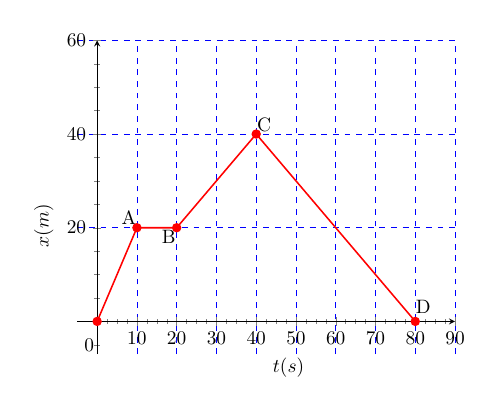
\begin{tikzpicture}[scale=0.7]
                \begin{axis}
                    [axis lines = left,
                    axis x line=center,
                    axis y line=center,
                    xlabel={$t(s)$},
                    ylabel={$x(m)$},
                    ylabel near ticks,
                    xlabel near ticks,
                    xlabel style={below right},
                    ylabel style={above left},
                    ymax=60,
                    ymin=-7,
                    xmax=90,
                    xmin=-5,
                    xtick={0,10,20,30,40,50,60,70,80,90},
                    ymajorgrids=true,
                    xmajorgrids=true,
                    minor tick num=3,
                    grid style={dashed, blue},
                    ]
                    \addplot[red,draw,thick, mark=*, mark options={fill=red}] coordinates {(0,0) (10,20) (20,20) (40,40) (80,0)};
                    \node at (axis cs:8,22) {A};
                    \draw (axis cs:10,20) circle;
                    \node at (axis cs:18,18) {B};
                    \node at (axis cs:42,42) {C};
                    \node at (axis cs:82,3) {D};
                    \node at (axis cs:-2,-5) {0};
                \end{axis}
        \end{tikzpicture}
        \caption{\textbf{Reference system}. Position vs time.}
    \end{figure}
\end{minipage}
% Additional text translation
\vspace*{-6pt}
\begin{itemize}[leftmargin=0pt]
        \item At \( t_B=\qty{20}{\s} \), the cyclist is also at \( x_B = \qty{20}{\metre} \).
        From \( t_B=10 \) to \( t_C=20 \), the displacement is \qty{0}{\m}, but total displacement from \( x_0 = 0 \) to \( x_B = 20 \) is \qty{20}{\m}.
        \item From \( x_C = 40 \) to \( x_D=0 \), the slope of the line is negative, indicating motion backward.
        The displacement from \( x_C = 40 \) to \( x_D = 0 \) is \qty{40}{\m} backward.
        From \( x_0 = 0 \) to \( x_D=80 \), the total displacement is \qty{0}{\m}.
        \item Total distance traveled is the sum of each segment: \( 20 + 0 + 20 + 40 = \qty{80}{\m} \).
\end{itemize}

\textbf{Motion analysis in each segment}:
\begin{itemize}
    \item Segment 0-A: URM (straight line on position-time graph)
    \item Segment A-B: No motion (object stationary)
    \item Segment B-C: URM again
    \item Segment C-D: URM backward
\end{itemize}
The graphs show the difference between displacement and distance travelled.
\section{Velocity-Time Graphs}
Velocity-time graphs represent the velocity of an object moving over a given period of time.
\begin{figure}[H]
    \centering
    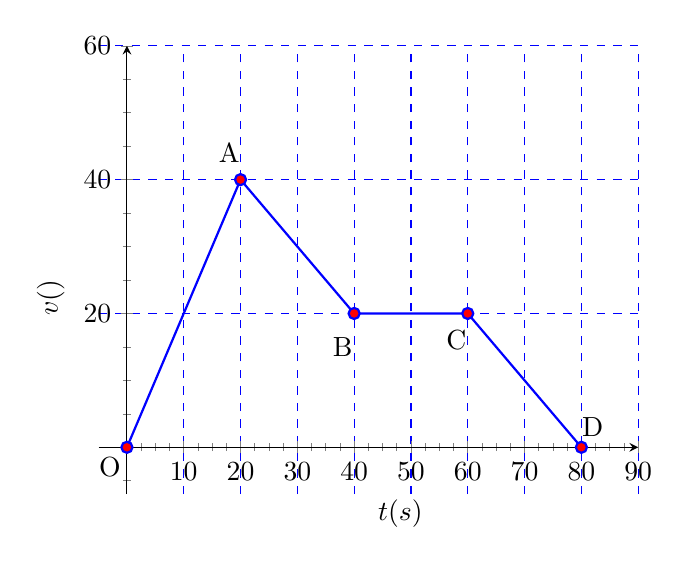
\begin{tikzpicture}[scale=1]
        \centering
        \begin{axis}
            [axis lines = left,
            axis x line=center,
            axis y line=center,
            mark=circle,
            xlabel={$t(s)$},
            ylabel={$v(\unit{\mps})$},
            ylabel near ticks,
            xlabel near ticks,
            xlabel style={below right},
            ylabel style={above left},
            ymax=60,
            ymin=-7,
            xmax=90,
            xmin=-5,
            xtick={0,10,20,30,40,50,60,70,80,90},
            ymajorgrids=true,
            xmajorgrids=true,
            minor tick num=3,
            grid style={dashed, blue},
            ]
            \addplot[blue,draw,thick, mark=*, mark options={fill=red}] coordinates {(0,0) (20,40) (40,20) (60,20) (80,0)};
            \node at (axis cs:18,44) {A};
            \draw (axis cs:10,20) circle;
            \node at (axis cs:38,15) {B};
            \node at (axis cs:58,16) {C};
            \node at (axis cs:82,3) {D};
            \node at (axis cs:-3,-3) {O};
        \end{axis}
    \end{tikzpicture}
    \caption{Graph of \( v \) vs \( t \)}
\end{figure}

\textbf{Analysis of the type of motion in the different segments:}

\begin{itemize}
    \item Segment O-A: We have a uniformly accelerated rectilinear motion (UARM) because the velocity-time graph is a straight line, and it moves forward.
    \item Segment A-B: We also have UARM, but now moving backward.
    \item Segment B-C: We have uniform rectilinear motion (URM) again because the velocity does not change, so the graph is horizontal.
    \item Segment C-D: Another UARM, now moving backward.
\end{itemize}


\begin{exercise}
    The graph below shows the motion of an object. Answer the following questions:
    \begin{enumerate}[label=\letraminuscula]
    \item What type of motion occurs in each section of the graph?
    \item Calculate the acceleration in each section.
    \item What is the total distance travelled by the object?
    \end{enumerate}

    \begin{figure}[H]
        \centering
        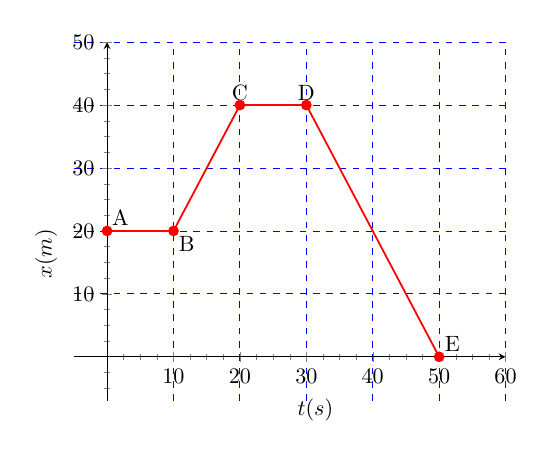
\begin{tikzpicture}[scale=0.8]
                \centering
                \begin{axis}
                    [axis lines = left,
                    axis x line=center,
                    axis y line=center,
                    mark=circle,
                    xlabel={$t(s)$},
                    ylabel={$x(m)$},
                    ylabel near ticks,
                    xlabel near ticks,
                    xlabel style={below right},
                    ylabel style={above left},
                    ymax=50,
                    ymin=-7,
                    xmax=60,
                    xmin=-5,
                    xtick={0,10,20,30,40,50,60},
                    ymajorgrids=true,
                    xmajorgrids=true,
                    minor tick num=3,
                    grid style={dashed, blue},
                    ]
                    \addplot[red,draw,thick, mark=*, mark options={fill=red}] coordinates {(0,20) (10,20) (20,40) (30,40) (50,0)};
                    \node at (axis cs:2,22) {A};
                    \draw (axis cs:10,20) circle;
                    \node at (axis cs:12,18) {B};
                    \node at (axis cs:20,42) {C};
                    \node at (axis cs:30,42) {D};
                    \node at (axis cs:52,2) {E};
                \end{axis}
        \end{tikzpicture}
    \end{figure}

    \begin{solu}
        \textbf{\textcolor{purple}{Exercise:}} The graph below shows the motion of an object. Answer the following questions:
        \begin{enumerate}[label=\letraminuscula]
            \item What type of motion occurs in each section of the graph?
            \item Calculate the acceleration in each section.
            \item What is the total distance travelled by the object?
        \end{enumerate}

        \vspace{0.3cm}

        \textcolor{blue}{Reading the graph:}
        \begin{itemize}
            \item Point A: $(0, 20)$ m
            \item Point B: $(10, 20)$ m
            \item Point C: $(20, 40)$ m
            \item Point D: $(30, 40)$ m
            \item Point E: $(50, 0)$ m
        \end{itemize}

        \textbf{\textcolor{blue}{Part a) Type of motion in each section}}

        \textcolor{blue}{Section A-B ($t = 0$ to $t = 10$ s):}
        \begin{itemize}
            \item Position remains constant at 20 m
            \item \textcolor{red}{Type: At rest (no motion, $v = 0$)}
        \end{itemize}

        \textcolor{blue}{Section B-C ($t = 10$ to $t = 20$ s):}
        \begin{itemize}
            \item Position increases linearly from 20 m to 40 m
            \item \textcolor{red}{Type: Uniform motion (constant positive velocity)}
        \end{itemize}

        \textcolor{blue}{Section C-D ($t = 20$ to $t = 30$ s):}
        \begin{itemize}
            \item Position remains constant at 40 m
            \item \textcolor{red}{Type: At rest (no motion, $v = 0$)}
        \end{itemize}

        \textcolor{blue}{Section D-E ($t = 30$ to $t = 50$ s):}
        \begin{itemize}
            \item Position decreases linearly from 40 m to 0 m
            \item \textcolor{red}{Type: Uniform motion (constant negative velocity - moving backward)}
        \end{itemize}

        \vspace{0.5cm}

        \textbf{\textcolor{blue}{Part b) Calculate acceleration in each section}}

        \textcolor{red}{Key concept:} Acceleration is the rate of change of velocity. For position-time graphs, acceleration is related to the curvature of the graph.

        \textcolor{blue}{Section A-B:}
        \[
            v = \frac{\Delta x}{\Delta t} = \frac{20 - 20}{10 - 0} = 0 \text{ m/s}
        \]
        Velocity is constant (zero), so: $\textcolor{red}{a = 0 \text{ m/s}^2}$

        \textcolor{blue}{Section B-C:}
        \[
            v = \frac{\Delta x}{\Delta t} = \frac{40 - 20}{20 - 10} = \frac{20}{10} = 2 \text{ m/s}
        \]
        Velocity is constant, so: $\textcolor{red}{a = 0 \text{ m/s}^2}$

        \textcolor{blue}{Section C-D:}
        \[
            v = \frac{\Delta x}{\Delta t} = \frac{40 - 40}{30 - 20} = 0 \text{ m/s}
        \]
        Velocity is constant (zero), so: $\textcolor{red}{a = 0 \text{ m/s}^2}$

        \textcolor{blue}{Section D-E:}
        \[
            v = \frac{\Delta x}{\Delta t} = \frac{0 - 40}{50 - 30} = \frac{-40}{20} = -2 \text{ m/s}
        \]
        Velocity is constant, so: $\textcolor{red}{a = 0 \text{ m/s}^2}$

        \textcolor{red}{Summary:} The acceleration is \textbf{zero} in all sections because the graph consists of straight line segments (constant velocity in each section). The velocity changes \textit{instantaneously} at points B, C, and D, which would require infinite acceleration, but this is an idealization.

        \vspace{0.5cm}

        \textbf{\textcolor{blue}{Part c) Total distance travelled}}

        \textcolor{red}{Important:} Distance is the total length of the path travelled (always positive), regardless of direction.

        \textcolor{blue}{Section A-B:}
        \[
            d_{AB} = |20 - 20| = 0 \text{ m}
        \]

        \textcolor{blue}{Section B-C:}
        \[
            d_{BC} = |40 - 20| = 20 \text{ m}
        \]

        \textcolor{blue}{Section C-D:}
        \[
            d_{CD} = |40 - 40| = 0 \text{ m}
        \]

        \textcolor{blue}{Section D-E:}
        \[
            d_{DE} = |0 - 40| = 40 \text{ m}
        \]

        \textcolor{blue}{Total distance:}
        \[
            d_{\text{total}} = d_{AB} + d_{BC} + d_{CD} + d_{DE}
        \]
        \[
            d_{\text{total}} = 0 + 20 + 0 + 40 = \textcolor{red}{60 \text{ m}}
        \]

        \textcolor{red}{Answer c):} The total distance travelled by the object is \textbf{60 m}.

        \textcolor{blue}{Note:} The displacement (change in position from start to finish) would be $0 - 20 = -20$ m, which is different from the total distance travelled.
    \end{solu}
\end{exercise}

\begin{exercise}
    The graph below shows the motion of an object. Answer the following questions:
    \begin{enumerate}[label=\letraminuscula]
    \item What type of motion occurs in each section of the graph?
    \item Calculate the acceleration in each section.
    \item What is the total distance travelled by the object?
    \end{enumerate}

    \begin{figure}[H]
        \centering
        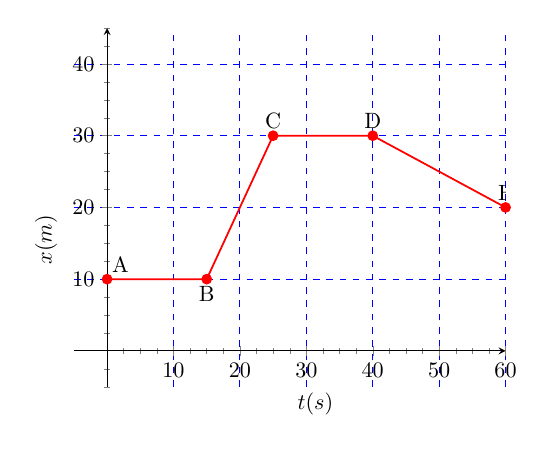
\begin{tikzpicture}[scale=0.8]
                \centering
                \begin{axis}
                    [axis lines = left,
                    axis x line=center,
                    axis y line=center,
                    xlabel={$t(s)$},
                    ylabel={$x(m)$},
                    ylabel near ticks,
                    xlabel near ticks,
                    xlabel style={below right},
                    ylabel style={above left},
                    ymax=45,
                    ymin=-5,
                    xmax=60,
                    xmin=-5,
                    xtick={0,10,20,30,40,50,60},
                    ymajorgrids=true,
                    xmajorgrids=true,
                    minor tick num=3,
                    grid style={dashed, blue},
                    ]
                    \addplot[red,draw,thick, mark=*, mark options={fill=red}] coordinates {(0,10) (15,10) (25,30) (40,30) (60,20)};
                    \node at (axis cs:2,12) {A};
                    \node at (axis cs:15,8) {B};
                    \node at (axis cs:25,32) {C};
                    \node at (axis cs:40,32) {D};
                    \node at (axis cs:60,22) {E};
                \end{axis}
        \end{tikzpicture}
    \end{figure}

    \begin{solu}
        \textbf{\textcolor{purple}{Exercise:}} The graph below shows the motion of an object. Answer the following questions:
        \begin{enumerate}[label=\letraminuscula]
            \item What type of motion occurs in each section of the graph?
            \item Calculate the acceleration in each section.
            \item What is the total distance travelled by the object?
        \end{enumerate}

        \vspace{0.3cm}

        \textcolor{blue}{Reading the graph:}
        \begin{itemize}
            \item Point A: $(0,10)$ m
            \item Point B: $(15,10)$ m
            \item Point C: $(25,30)$ m
            \item Point D: $(40,30)$ m
            \item Point E: $(60,20)$ m
        \end{itemize}

        \textbf{\textcolor{blue}{Part a) Type of motion in each section}}

        \textcolor{blue}{Section A-B ($t=0$ to $15$ s):}
        \begin{itemize}
            \item Position remains constant.
            \item \textcolor{red}{Type: At rest ($v=0$).}
        \end{itemize}

        \textcolor{blue}{Section B-C ($t=15$ to $25$ s):}
        \begin{itemize}
            \item Position increases linearly.
            \item \textcolor{red}{Type: Uniform motion (constant positive velocity).}
        \end{itemize}

        \textcolor{blue}{Section C-D ($t=25$ to $40$ s):}
        \begin{itemize}
            \item Position remains constant.
            \item \textcolor{red}{Type: At rest ($v=0$).}
        \end{itemize}

        \textcolor{blue}{Section D-E ($t=40$ to $60$ s):}
        \begin{itemize}
            \item Position decreases linearly.
            \item \textcolor{red}{Type: Uniform motion (constant negative velocity).}
        \end{itemize}

        \vspace{0.5cm}

        \textbf{\textcolor{blue}{Part b) Calculate acceleration in each section}}

        \textcolor{blue}{Section A-B:}
        \[
        v=\frac{10-10}{15-0}=0\text{ m/s}
        \]
        Therefore,
        \[
        \boxed{a=0\text{ m/s}^2}
        \]

        \textcolor{blue}{Section B-C:}
        \[
        v=\frac{30-10}{25-15}=\frac{20}{10}=2\text{ m/s}
        \]
        Therefore,
        \[
        \boxed{a=0\text{ m/s}^2}
        \]

        \textcolor{blue}{Section C-D:}
        \[
        v=\frac{30-30}{40-25}=0\text{ m/s}
        \]
        Therefore,
        \[
        \boxed{a=0\text{ m/s}^2}
        \]

        \textcolor{blue}{Section D-E:}
        \[
        v=\frac{20-30}{60-40}=\frac{-10}{20}=-0.5\text{ m/s}
        \]
        Therefore,
        \[
        \boxed{a=0\text{ m/s}^2}
        \]

        \textcolor{red}{Acceleration is zero in every section because the velocity is constant in each interval.}

        \vspace{0.5cm}

        \textbf{\textcolor{blue}{Part c) Total distance travelled}}

        \[
        d_{AB}=0\text{ m}
        \]

        \[
        d_{BC}=20\text{ m}
        \]

        \[
        d_{CD}=0\text{ m}
        \]

        \[
        d_{DE}=10\text{ m}
        \]

        \[
        d_{\text{total}}=0+20+0+10=\boxed{30\text{ m}}
        \]

        \textcolor{blue}{The displacement is $20-10=10$ m.}
    \end{solu}
\end{exercise}

\begin{exercise}
    The graph below shows the motion of an object. Answer the following questions:
    \begin{enumerate}[label=\letraminuscula]
    \item What type of motion occurs in each section of the graph?
    \item Calculate the acceleration in each section.
    \item What is the total distance travelled by the object?
    \end{enumerate}

    \begin{figure}[H]
        \centering
        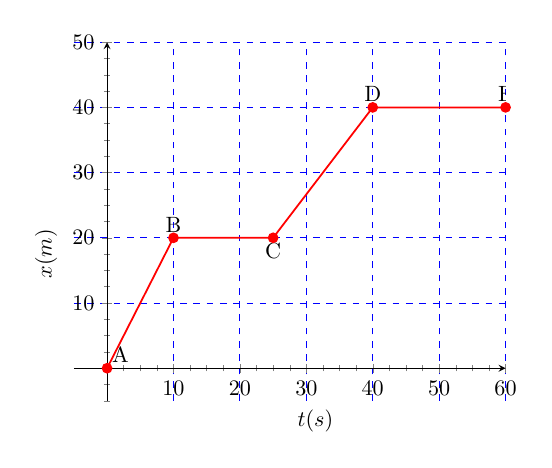
\begin{tikzpicture}[scale=0.8]
                \centering
                \begin{axis}
                    [axis lines = left,
                    axis x line=center,
                    axis y line=center,
                    xlabel={$t(s)$},
                    ylabel={$x(m)$},
                    ylabel near ticks,
                    xlabel near ticks,
                    xlabel style={below right},
                    ylabel style={above left},
                    ymax=50,
                    ymin=-5,
                    xmax=60,
                    xmin=-5,
                    xtick={0,10,20,30,40,50,60},
                    ymajorgrids=true,
                    xmajorgrids=true,
                    minor tick num=3,
                    grid style={dashed, blue},
                    ]
                    \addplot[red,draw,thick, mark=*, mark options={fill=red}] coordinates {(0,0) (10,20) (25,20) (40,40) (60,40)};
                    \node at (axis cs:2,2) {A};
                    \node at (axis cs:10,22) {B};
                    \node at (axis cs:25,18) {C};
                    \node at (axis cs:40,42) {D};
                    \node at (axis cs:60,42) {E};
                \end{axis}
        \end{tikzpicture}
    \end{figure}

    \begin{solu}
        \textbf{\textcolor{purple}{Exercise:}} The graph below shows the motion of an object. Answer the following questions:
        \begin{enumerate}[label=\letraminuscula]
            \item What type of motion occurs in each section of the graph?
            \item Calculate the acceleration in each section.
            \item What is the total distance travelled by the object?
        \end{enumerate}

        \vspace{0.3cm}

        \textcolor{blue}{Reading the graph:}
        \begin{itemize}
            \item Point A: $(0,0)$ m
            \item Point B: $(10,20)$ m
            \item Point C: $(25,20)$ m
            \item Point D: $(40,40)$ m
            \item Point E: $(60,40)$ m
        \end{itemize}

        \textbf{\textcolor{blue}{Part a) Type of motion in each section}}

        \textcolor{blue}{Section A-B:}
        \begin{itemize}
            \item Position increases linearly.
            \item \textcolor{red}{Type: Uniform motion (constant positive velocity).}
        \end{itemize}

        \textcolor{blue}{Section B-C:}
        \begin{itemize}
            \item Position remains constant.
            \item \textcolor{red}{Type: At rest.}
        \end{itemize}

        \textcolor{blue}{Section C-D:}
        \begin{itemize}
            \item Position increases linearly.
            \item \textcolor{red}{Type: Uniform motion (constant positive velocity).}
        \end{itemize}

        \textcolor{blue}{Section D-E:}
        \begin{itemize}
            \item Position remains constant.
            \item \textcolor{red}{Type: At rest.}
        \end{itemize}

        \vspace{0.5cm}

        \textbf{\textcolor{blue}{Part b) Calculate acceleration in each section}}

        \textcolor{blue}{Section A-B:}
        \[
        v=\frac{20-0}{10-0}=2\text{ m/s}
        \]
        Therefore,
        \[
        \boxed{a=0\text{ m/s}^2}
        \]

        \textcolor{blue}{Section B-C:}
        \[
        v=\frac{20-20}{25-10}=0\text{ m/s}
        \]
        Therefore,
        \[
        \boxed{a=0\text{ m/s}^2}
        \]

        \textcolor{blue}{Section C-D:}
        \[
        v=\frac{40-20}{40-25}=\frac{20}{15}=1.33\text{ m/s}
        \]
        Therefore,
        \[
        \boxed{a=0\text{ m/s}^2}
        \]

        \textcolor{blue}{Section D-E:}
        \[
        v=\frac{40-40}{60-40}=0\text{ m/s}
        \]
        Therefore,
        \[
        \boxed{a=0\text{ m/s}^2}
        \]

        \textcolor{red}{Acceleration is zero in all sections because every segment is a straight line.}

        \vspace{0.5cm}

        \textbf{\textcolor{blue}{Part c) Total distance travelled}}

        \[
        d_{AB}=20\text{ m}
        \]

        \[
        d_{BC}=0\text{ m}
        \]

        \[
        d_{CD}=20\text{ m}
        \]

        \[
        d_{DE}=0\text{ m}
        \]

        \[
        d_{\text{total}}=20+0+20+0=\boxed{40\text{ m}}
        \]

        \textcolor{blue}{The displacement is $40-0=40$ m.}
    \end{solu}
\end{exercise}

\begin{exercise}
    The graph below shows the velocity of an object. Answer the following questions:
    \begin{enumerate}[label=\letraminuscula]
    \item What type of motion occurs in each section of the graph?
    \item Calculate the acceleration in each section.
    \item What is the total distance travelled by the object?
    \end{enumerate}

    \begin{figure}[H]
        \centering
        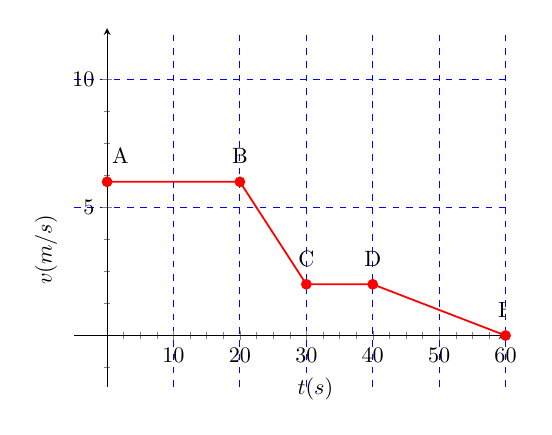
\begin{tikzpicture}[scale=0.8]
            \begin{axis}
                [axis lines = left,
                axis x line=center,
                axis y line=center,
                xlabel={$t(s)$},
                ylabel={$v(m/s)$},
                ylabel near ticks,
                xlabel near ticks,
                xlabel style={below right},
                ylabel style={above left},
                ymax=12,
                ymin=-2,
                xmax=60,
                xmin=-5,
                xtick={0,10,20,30,40,50,60},
                ymajorgrids=true,
                xmajorgrids=true,
                minor tick num=3,
                grid style={dashed, blue},
                ]
                \addplot[red,draw,thick,mark=*,mark options={fill=red}]
                coordinates {(0,6) (20,6) (30,2) (40,2) (60,0)};
                \node at (axis cs:2,7) {A};
                \node at (axis cs:20,7) {B};
                \node at (axis cs:30,3) {C};
                \node at (axis cs:40,3) {D};
                \node at (axis cs:60,1) {E};
            \end{axis}
        \end{tikzpicture}
    \end{figure}

    \begin{solu}

    \textbf{\textcolor{purple}{Exercise:}} The graph below shows the velocity of an object.

    \textcolor{blue}{Reading the graph:}
    \begin{itemize}
        \item A: $(0,6)$ m/s
        \item B: $(20,6)$ m/s
        \item C: $(30,2)$ m/s
        \item D: $(40,2)$ m/s
        \item E: $(60,0)$ m/s
    \end{itemize}

    \textbf{\textcolor{blue}{Part a) Type of motion}}

    \textbf{A-B:}
    \begin{itemize}
        \item Constant velocity.
        \item \textcolor{red}{Uniform motion.}
    \end{itemize}

    \textbf{B-C:}
    \begin{itemize}
        \item Velocity decreases uniformly.
        \item \textcolor{red}{Uniformly decelerated motion.}
    \end{itemize}

    \textbf{C-D:}
    \begin{itemize}
        \item Constant velocity.
        \item \textcolor{red}{Uniform motion.}
    \end{itemize}

    \textbf{D-E:}
    \begin{itemize}
        \item Velocity decreases uniformly.
        \item \textcolor{red}{Uniformly decelerated motion.}
    \end{itemize}

    \textbf{\textcolor{blue}{Part b) Acceleration}}

    A-B:
    \[
    a=\frac{6-6}{20}=0\text{ m/s}^2
    \]

    B-C:
    \[
    a=\frac{2-6}{10}=-0.4\text{ m/s}^2
    \]

    C-D:
    \[
    a=\frac{2-2}{10}=0\text{ m/s}^2
    \]

    D-E:
    \[
    a=\frac{0-2}{20}=-0.1\text{ m/s}^2
    \]

    \textbf{\textcolor{blue}{Part c) Total distance}}

    Area A-B:
    \[
    (20)(6)=120\text{ m}
    \]

    Area B-C:
    \[
    \frac{6+2}{2}(10)=40\text{ m}
    \]

    Area C-D:
    \[
    (10)(2)=20\text{ m}
    \]

    Area D-E:
    \[
    \frac{2+0}{2}(20)=20\text{ m}
    \]

    Total distance:
    \[
    d=120+40+20+20=\boxed{200\text{ m}}
    \]

    \end{solu}
\end{exercise}

\begin{exercise}
    The graph below shows the velocity of an object. Answer the following questions:
    \begin{enumerate}[label=\letraminuscula]
    \item What type of motion occurs in each section of the graph?
    \item Calculate the acceleration in each section.
    \item What is the total distance travelled by the object?
    \end{enumerate}

    \begin{figure}[H]
        \centering
        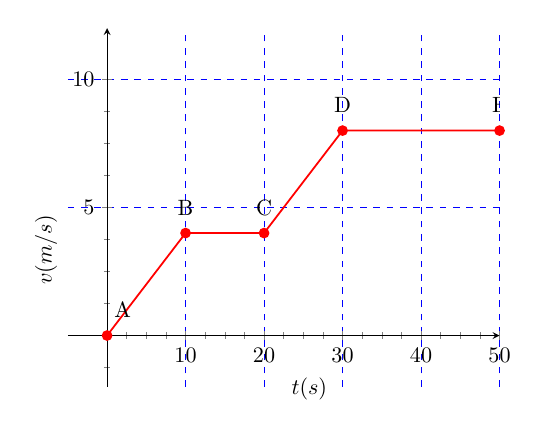
\begin{tikzpicture}[scale=0.8]
            \begin{axis}
                [axis lines = left,
                axis x line=center,
                axis y line=center,
                xlabel={$t(s)$},
                ylabel={$v(m/s)$},
                ylabel near ticks,
                xlabel near ticks,
                xlabel style={below right},
                ylabel style={above left},
                ymax=12,
                ymin=-2,
                xmax=50,
                xmin=-5,
                xtick={0,10,20,30,40,50},
                ymajorgrids=true,
                xmajorgrids=true,
                minor tick num=3,
                grid style={dashed, blue},
                ]
                \addplot[red,draw,thick,mark=*,mark options={fill=red}]
                coordinates {(0,0) (10,4) (20,4) (30,8) (50,8)};
                \node at (axis cs:2,1) {A};
                \node at (axis cs:10,5) {B};
                \node at (axis cs:20,5) {C};
                \node at (axis cs:30,9) {D};
                \node at (axis cs:50,9) {E};
            \end{axis}
        \end{tikzpicture}
    \end{figure}

    \begin{solu}

    \textbf{\textcolor{purple}{Exercise:}} The graph below shows the velocity of an object.

    \textcolor{blue}{Reading the graph:}
    \begin{itemize}
        \item A: $(0,0)$ m/s
        \item B: $(10,4)$ m/s
        \item C: $(20,4)$ m/s
        \item D: $(30,8)$ m/s
        \item E: $(50,8)$ m/s
    \end{itemize}

    \textbf{\textcolor{blue}{Part a) Type of motion}}

    \textbf{A-B:}
    \begin{itemize}
        \item Velocity increases uniformly.
        \item \textcolor{red}{Uniformly accelerated motion.}
    \end{itemize}

    \textbf{B-C:}
    \begin{itemize}
        \item Constant velocity.
        \item \textcolor{red}{Uniform motion.}
    \end{itemize}

    \textbf{C-D:}
    \begin{itemize}
        \item Velocity increases uniformly.
        \item \textcolor{red}{Uniformly accelerated motion.}
    \end{itemize}

    \textbf{D-E:}
    \begin{itemize}
        \item Constant velocity.
        \item \textcolor{red}{Uniform motion.}
    \end{itemize}

    \textbf{\textcolor{blue}{Part b) Acceleration}}

    A-B:
    \[
    a=\frac{4-0}{10}=0.4\text{ m/s}^2
    \]

    B-C:
    \[
    a=\frac{4-4}{10}=0\text{ m/s}^2
    \]

    C-D:
    \[
    a=\frac{8-4}{10}=0.4\text{ m/s}^2
    \]

    D-E:
    \[
    a=\frac{8-8}{20}=0\text{ m/s}^2
    \]

    \textbf{\textcolor{blue}{Part c) Total distance}}

    Area A-B:
    \[
    \frac12(10)(4)=20\text{ m}
    \]

    Area B-C:
    \[
    (10)(4)=40\text{ m}
    \]

    Area C-D:
    \[
    \frac{4+8}{2}(10)=60\text{ m}
    \]

    Area D-E:
    \[
    (20)(8)=160\text{ m}
    \]

    Total distance:
    \[
    d=20+40+60+160=\boxed{280\text{ m}}
    \]

    \end{solu}
\end{exercise}

\begin{exercise}
    Create a concept map summarising the main topics of this unit.
    \begin{solu}
        \textbf{\textcolor{purple}{Exercise:}} Create a concept map summarising the main topics of this unit.

        \textcolor{blue}{This is an open-ended exercise where students should create their own concept map including key terms such as: position, displacement, velocity, speed, acceleration, uniform motion, uniformly accelerated motion, position-time graphs, velocity-time graphs, kinematic equations, etc.}
    \end{solu}
\end{exercise}

\section{Vocabulary}

\begin{vocabulary}[Kinematics]
The branch of Physics that studies motion without taking into account the causes that produce it. It focuses on describing how objects move through space and time. \newline
\textbf{Translation to Spanish}: Cinemática \newline
% Line 9
\end{vocabulary}

\begin{vocabulary}[Motion]
The change in position of an object with respect to a reference system over time. An object is in motion when its position changes relative to a chosen reference point. \newline
\textbf{Translation to Spanish}: Movimiento \newline
% Line 49
\end{vocabulary}

\begin{vocabulary}[Rest]
The state of an object when its position does not change with respect to a reference system over time. \newline
\textbf{Translation to Spanish}: Reposo \newline
% Line 51
\end{vocabulary}

\begin{vocabulary}[Reference System]
A system that allows us to fix the position of an object and study its evolution over time. In Physics, it is usually a Cartesian coordinate system (x, y). \newline
\textbf{Translation to Spanish}: Sistema de referencia \newline
% Line 58
\end{vocabulary}

\begin{vocabulary}[Position]
The exact location of an object in space, usually represented by the letter x. The SI unit is the meter (m). \newline
\textbf{Translation to Spanish}: Posición \newline
% Line 69
\end{vocabulary}

\begin{vocabulary}[Displacement]
The difference between the final position and the initial position of the motion, represented as \( \Delta x = x_f - x_i \). It is a vector quantity that can be positive or negative. The SI unit is the meter (m). \newline
\textbf{Translation to Spanish}: Desplazamiento \newline
% Line 73
\end{vocabulary}

\begin{vocabulary}[Trajectory]
The path followed by an object during its motion. It can be rectilinear (straight line), circular, or curvilinear (curved). \newline
\textbf{Translation to Spanish}: Trayectoria \newline
% Line 103
\end{vocabulary}

\begin{vocabulary}[Distance Travelled]
The length of the trajectory followed by an object. It is a scalar quantity always positive. The SI unit is the meter (m). \newline
\textbf{Translation to Spanish}: Distancia recorrida \newline
% Line 106
\end{vocabulary}

\begin{vocabulary}[Rectilinear Motion]
Motion in which the trajectory is a straight line. In this type of motion, displacement coincides with the distance traveled. \newline
\textbf{Translation to Spanish}: Movimiento rectilíneo \newline
% Line 114
\end{vocabulary}

\begin{vocabulary}[Circular Motion]
Motion in which the trajectory is circular or describes a circle. \newline
\textbf{Translation to Spanish}: Movimiento circular \newline
% Line 117
\end{vocabulary}

\begin{vocabulary}[Curvilinear Motion]
Motion in which the trajectory describes curves that are neither straight lines nor perfect circles. \newline
\textbf{Translation to Spanish}: Movimiento curvilíneo \newline
% Line 119
\end{vocabulary}

\begin{vocabulary}[Velocity]
The rate of change of position with respect to time. It is a vector quantity that indicates both speed and direction. The SI unit is meters per second (m/s). \newline
\textbf{Translation to Spanish}: Velocidad \newline
% Line 201 (approximately, appears throughout the document)
\end{vocabulary}

\begin{vocabulary}[Speed]
The magnitude of velocity, representing how fast an object is moving without regard to direction. It is a scalar quantity. The SI unit is meters per second (m/s). \newline
\textbf{Translation to Spanish}: Rapidez \newline
% Line 201 (approximately, appears throughout the document)
\end{vocabulary}

\begin{vocabulary}[Average Velocity]
The total displacement divided by the total time taken. It is calculated as \( v_{avg} = \Delta x / \Delta t \) \newline
\textbf{Translation to Spanish}: Velocidad media \newline
% Line 201 (approximately, appears in context)
\end{vocabulary}

\begin{vocabulary}[Instantaneous Velocity]
The velocity of an object at a specific instant of time. It is the limit of average velocity as the time interval approaches zero. \newline
\textbf{Translation to Spanish}: Velocidad instantánea \newline
% Line 201 (approximately, appears in context)
\end{vocabulary}

\begin{vocabulary}[Acceleration]
The rate of change of velocity with respect to time. It is a vector quantity. The SI unit is meters per second squared (m/s²). \newline
\textbf{Translation to Spanish}: Aceleración \newline
% Line 201 (approximately, appears throughout the document)
\end{vocabulary}

\begin{vocabulary}[Uniform Rectilinear Motion (URM)]
Motion in a straight line with constant velocity (zero acceleration). The object covers equal distances in equal time intervals. \newline
\textbf{Translation to Spanish}: Movimiento rectilíneo uniforme (MRU) \newline
% Line 2346
\end{vocabulary}

\begin{vocabulary}[Uniformly Accelerated Rectilinear Motion (UARM)]
Motion in a straight line with constant acceleration. The velocity changes uniformly over time. Also known as uniformly varied motion. \newline
\textbf{Translation to Spanish}: Movimiento rectilíneo uniformemente acelerado (MRUA) \newline
% Line 2399
\end{vocabulary}

\begin{vocabulary}[Coordinate System]
A system used to specify the position of a point in space using numerical coordinates. The most common is the Cartesian coordinate system. \newline
\textbf{Translation to Spanish}: Sistema de coordenadas \newline
% Line 55
\end{vocabulary}

\begin{vocabulary}[Origin]
The reference point in a coordinate system where all coordinates are zero. It serves as the starting point for measuring position. \newline
\textbf{Translation to Spanish}: Origen \newline
% Line 2288
\end{vocabulary}

\begin{vocabulary}[Time Interval]
The difference between two moments in time, calculated as \( \Delta t = t_f - t_i \). It represents the duration of an event or motion. \newline
\textbf{Translation to Spanish}: Intervalo de tiempo \newline
% Line 94
\end{vocabulary}

\begin{vocabulary}[Position-Time Graph]
A graphical representation showing how an object's position changes over time. The slope of the graph represents velocity. \newline
\textbf{Translation to Spanish}: Gráfica posición-tiempo \newline
% Line 2283
\end{vocabulary}

\begin{vocabulary}[Velocity-Time Graph]
A graphical representation showing how an object's velocity changes over time. The slope represents acceleration, and the area under the curve represents displacement. \newline
\textbf{Translation to Spanish}: Gráfica velocidad-tiempo \newline
% Line 2355
\end{vocabulary}

\begin{vocabulary}[Slope]
In a graph, the slope represents the rate of change of the vertical quantity with respect to the horizontal quantity. In position-time graphs, slope represents velocity; in velocity-time graphs, it represents acceleration. \newline
\textbf{Translation to Spanish}: Pendiente \newline
% Line 2337
\end{vocabulary}

\begin{vocabulary}[Vector Quantity]
A physical quantity that has both magnitude and direction. Examples include displacement, velocity, and acceleration. \newline
\textbf{Translation to Spanish}: Magnitud vectorial \newline
% Line 159
\end{vocabulary}

\begin{vocabulary}[Scalar Quantity]
A physical quantity that has only magnitude but no direction. Examples include distance, speed, and time. \newline
\textbf{Translation to Spanish}: Magnitud escalar \newline
% Line 107 (implied in context)
\end{vocabulary}

\begin{vocabulary}[Initial Position]
The position of an object at the beginning of motion or at the start of observation, represented as \( x_i \) or \(v  \). \newline
\textbf{Translation to Spanish}: Posición inicial \newline
% Line 83
\end{vocabulary}

\begin{vocabulary}[Final Position]
The position of an object at the end of motion or at a specific moment, represented as \( x_f \) . \newline
\textbf{Translation to Spanish}: Posición final \newline
% Line 81
\end{vocabulary}

\begin{vocabulary}[Cartesian Coordinate System]
A coordinate system that uses perpendicular axes (typically x and y in 2D, or x, y, and z in 3D) to specify positions in space. \newline
\textbf{Translation to Spanish}: Sistema de coordenadas cartesianas \newline
% Line 55
\end{vocabulary}

\begin{vocabulary}[Frame of Reference]
A perspective from which motion is observed and measured. Motion is relative and depends on the chosen frame of reference. \newline
\textbf{Translation to Spanish}: Sistema de referencia \newline
% Line 53
\end{vocabulary}


%\begin{exercise}
%    Vocabulary
%
%    \begin{multicols}{2}
%        \begin{enumerate}
%            \item Acceleration
%            \item at rest
%            \item Average
%            \item Axis
%            \item Coordinate System
%            \item Deform
%            \item Direction
%            \item displacement
%            \item Frame of reference
%            \item Instantaneous
%            \item Interval
%            \item Law
%            \item Motion
%            \item Origin
%            \item Slope
%            \item Speed
%            \item Trajectory
%            \item Uniform rectilinear motion.
%        \end{enumerate}
%    \end{multicols}

%\end{exercise}


